\documentclass[]{tufte-book}

% ams
\usepackage{amssymb,amsmath}

\usepackage{ifxetex,ifluatex}
\usepackage{fixltx2e} % provides \textsubscript
\ifnum 0\ifxetex 1\fi\ifluatex 1\fi=0 % if pdftex
  \usepackage[T1]{fontenc}
  \usepackage[utf8]{inputenc}
\else % if luatex or xelatex
  \makeatletter
  \@ifpackageloaded{fontspec}{}{\usepackage{fontspec}}
  \makeatother
  \defaultfontfeatures{Ligatures=TeX,Scale=MatchLowercase}
  \makeatletter
  \@ifpackageloaded{soul}{
     \renewcommand\allcapsspacing[1]{{\addfontfeature{LetterSpace=15}#1}}
     \renewcommand\smallcapsspacing[1]{{\addfontfeature{LetterSpace=10}#1}}
   }{}
  \makeatother

\fi

% graphix
\usepackage{graphicx}
\setkeys{Gin}{width=\linewidth,totalheight=\textheight,keepaspectratio}

% booktabs
\usepackage{booktabs}

% url
\usepackage{url}

% hyperref
\usepackage{hyperref}

% units.
\usepackage{units}


\setcounter{secnumdepth}{2}

% citations
\usepackage{natbib}
\bibliographystyle{apalike}

% pandoc syntax highlighting
\usepackage{color}
\usepackage{fancyvrb}
\newcommand{\VerbBar}{|}
\newcommand{\VERB}{\Verb[commandchars=\\\{\}]}
\DefineVerbatimEnvironment{Highlighting}{Verbatim}{commandchars=\\\{\}}
% Add ',fontsize=\small' for more characters per line
\newenvironment{Shaded}{}{}
\newcommand{\KeywordTok}[1]{\textcolor[rgb]{0.00,0.44,0.13}{\textbf{#1}}}
\newcommand{\DataTypeTok}[1]{\textcolor[rgb]{0.56,0.13,0.00}{#1}}
\newcommand{\DecValTok}[1]{\textcolor[rgb]{0.25,0.63,0.44}{#1}}
\newcommand{\BaseNTok}[1]{\textcolor[rgb]{0.25,0.63,0.44}{#1}}
\newcommand{\FloatTok}[1]{\textcolor[rgb]{0.25,0.63,0.44}{#1}}
\newcommand{\ConstantTok}[1]{\textcolor[rgb]{0.53,0.00,0.00}{#1}}
\newcommand{\CharTok}[1]{\textcolor[rgb]{0.25,0.44,0.63}{#1}}
\newcommand{\SpecialCharTok}[1]{\textcolor[rgb]{0.25,0.44,0.63}{#1}}
\newcommand{\StringTok}[1]{\textcolor[rgb]{0.25,0.44,0.63}{#1}}
\newcommand{\VerbatimStringTok}[1]{\textcolor[rgb]{0.25,0.44,0.63}{#1}}
\newcommand{\SpecialStringTok}[1]{\textcolor[rgb]{0.73,0.40,0.53}{#1}}
\newcommand{\ImportTok}[1]{#1}
\newcommand{\CommentTok}[1]{\textcolor[rgb]{0.38,0.63,0.69}{\textit{#1}}}
\newcommand{\DocumentationTok}[1]{\textcolor[rgb]{0.73,0.13,0.13}{\textit{#1}}}
\newcommand{\AnnotationTok}[1]{\textcolor[rgb]{0.38,0.63,0.69}{\textbf{\textit{#1}}}}
\newcommand{\CommentVarTok}[1]{\textcolor[rgb]{0.38,0.63,0.69}{\textbf{\textit{#1}}}}
\newcommand{\OtherTok}[1]{\textcolor[rgb]{0.00,0.44,0.13}{#1}}
\newcommand{\FunctionTok}[1]{\textcolor[rgb]{0.02,0.16,0.49}{#1}}
\newcommand{\VariableTok}[1]{\textcolor[rgb]{0.10,0.09,0.49}{#1}}
\newcommand{\ControlFlowTok}[1]{\textcolor[rgb]{0.00,0.44,0.13}{\textbf{#1}}}
\newcommand{\OperatorTok}[1]{\textcolor[rgb]{0.40,0.40,0.40}{#1}}
\newcommand{\BuiltInTok}[1]{#1}
\newcommand{\ExtensionTok}[1]{#1}
\newcommand{\PreprocessorTok}[1]{\textcolor[rgb]{0.74,0.48,0.00}{#1}}
\newcommand{\AttributeTok}[1]{\textcolor[rgb]{0.49,0.56,0.16}{#1}}
\newcommand{\RegionMarkerTok}[1]{#1}
\newcommand{\InformationTok}[1]{\textcolor[rgb]{0.38,0.63,0.69}{\textbf{\textit{#1}}}}
\newcommand{\WarningTok}[1]{\textcolor[rgb]{0.38,0.63,0.69}{\textbf{\textit{#1}}}}
\newcommand{\AlertTok}[1]{\textcolor[rgb]{1.00,0.00,0.00}{\textbf{#1}}}
\newcommand{\ErrorTok}[1]{\textcolor[rgb]{1.00,0.00,0.00}{\textbf{#1}}}
\newcommand{\NormalTok}[1]{#1}

% longtable
\usepackage{longtable,booktabs}

% multiplecol
\usepackage{multicol}

% strikeout
\usepackage[normalem]{ulem}

% morefloats
\usepackage{morefloats}


% tightlist macro required by pandoc >= 1.14
\providecommand{\tightlist}{%
  \setlength{\itemsep}{0pt}\setlength{\parskip}{0pt}}

% title / author / date
\title{R für die sozio-ökonomische Forschung}
\author{\href{http://claudius-graebner.com/}{Dr.~Claudius Gräbner}}
\date{2019-11-03}

\usepackage{booktabs}
\usepackage{amsthm, amssymb, mathrsfs}
\usepackage{xcolor}
\usepackage{hyperref}
\hypersetup{
    colorlinks = true,
    linkcolor = {blue},
    citecolor = {violet}}
%\usepackage[top=2cm, bottom=2cm, left=2cm, right=4cm]{geometry}
\makeatletter
\def\thm@space@setup{%
  \thm@preskip=8pt plus 2pt minus 4pt
  \thm@postskip=\thm@preskip
}
\makeatother

\begin{document}

\maketitle



{
\setcounter{tocdepth}{1}
\tableofcontents
}

\chapter*{Willkommen}\label{willkommen}
\addcontentsline{toc}{chapter}{Willkommen}

Dieses Skript ist als Begleitung für die Lehrveranstaltung
``Wissenschaftstheorie und Einführung in die Methoden der
Sozioökonomie'' im Master ``Sozioökonomie'' an der Universität
Duisburg-Essen gedacht.

Es enthält grundlegende Informationen über die Funktion der
Programmiersprache R \citep{R-Team}.

\section*{Verhältnis zur Vorlesung}\label{verhaltnis-zur-vorlesung}
\addcontentsline{toc}{section}{Verhältnis zur Vorlesung}

Einige Kapitel beziehen sich unmittelbar auf bestimmte
Vorlesungstermine, andere sind als optionale Zusatzinformation gedacht.
Gerade Menschen ohne Vorkenntnisse in R sollten unbedingt die ersten
Kapitel vor dem vierten Vorlesungsterm lesen und verstehen. Bei Fragen
können Sie sich gerne an Claudius Gräbner wenden.

Die folgende Tabelle gibt einen Überblick über die Kapitel und die
dazugehörigen Vorlesungstermine:

\begin{longtable}[]{@{}clc@{}}
\toprule
\begin{minipage}[b]{0.24\columnwidth}\centering\strut
Kapitel\strut
\end{minipage} & \begin{minipage}[b]{0.34\columnwidth}\raggedright\strut
Zentrale Inhalte\strut
\end{minipage} & \begin{minipage}[b]{0.34\columnwidth}\centering\strut
Verwandter Vorlesungstermin\strut
\end{minipage}\tabularnewline
\midrule
\endhead
\begin{minipage}[t]{0.24\columnwidth}\centering\strut
1: Vorbemerkungen\strut
\end{minipage} & \begin{minipage}[t]{0.34\columnwidth}\raggedright\strut
Gründe für R; Besonderheiten von R\strut
\end{minipage} & \begin{minipage}[t]{0.34\columnwidth}\centering\strut
Vorbereitung\strut
\end{minipage}\tabularnewline
\begin{minipage}[t]{0.24\columnwidth}\centering\strut
2: Vorbereitung\strut
\end{minipage} & \begin{minipage}[t]{0.34\columnwidth}\raggedright\strut
Installation und Einrichtung von R und R Studio,
Projektstrukturierung\strut
\end{minipage} & \begin{minipage}[t]{0.34\columnwidth}\centering\strut
Vorbereitung\strut
\end{minipage}\tabularnewline
\begin{minipage}[t]{0.24\columnwidth}\centering\strut
3: Erste Schritte in R\strut
\end{minipage} & \begin{minipage}[t]{0.34\columnwidth}\raggedright\strut
Grundlegende Funktionen von R; Objekte in R; Pakete\strut
\end{minipage} & \begin{minipage}[t]{0.34\columnwidth}\centering\strut
Vorbereitung\strut
\end{minipage}\tabularnewline
\begin{minipage}[t]{0.24\columnwidth}\centering\strut
4: Ökonometrie I\strut
\end{minipage} & \begin{minipage}[t]{0.34\columnwidth}\raggedright\strut
Implementierung von uni- und multivariaten linearen
Regressionsmodellen\strut
\end{minipage} & \begin{minipage}[t]{0.34\columnwidth}\centering\strut
T4 am 06.11.19\strut
\end{minipage}\tabularnewline
\begin{minipage}[t]{0.24\columnwidth}\centering\strut
5: Datenaquise und -management\strut
\end{minipage} & \begin{minipage}[t]{0.34\columnwidth}\raggedright\strut
Einlesen und Schreiben sowie Manipulation von Datensätzen; deskriptive
Statistik\strut
\end{minipage} & \begin{minipage}[t]{0.34\columnwidth}\centering\strut
T8 am 11.12.19\strut
\end{minipage}\tabularnewline
\begin{minipage}[t]{0.24\columnwidth}\centering\strut
6: Visualisierung\strut
\end{minipage} & \begin{minipage}[t]{0.34\columnwidth}\raggedright\strut
Erstellen von Grafiken\strut
\end{minipage} & \begin{minipage}[t]{0.34\columnwidth}\centering\strut
T8 am 11.12.19\strut
\end{minipage}\tabularnewline
\begin{minipage}[t]{0.24\columnwidth}\centering\strut
7: Ökonometrie II\strut
\end{minipage} & \begin{minipage}[t]{0.34\columnwidth}\raggedright\strut
Mehr Konzepte der Ökonometrie\strut
\end{minipage} & \begin{minipage}[t]{0.34\columnwidth}\centering\strut
T9-10 am 8.\&15.1.20\strut
\end{minipage}\tabularnewline
\begin{minipage}[t]{0.24\columnwidth}\centering\strut
8: Ausblick\strut
\end{minipage} & \begin{minipage}[t]{0.34\columnwidth}\raggedright\strut
Ausblick zu weiteren Anwendungsmöglichkeiten\strut
\end{minipage} & \begin{minipage}[t]{0.34\columnwidth}\centering\strut
Optional\strut
\end{minipage}\tabularnewline
\begin{minipage}[t]{0.24\columnwidth}\centering\strut
A: Einführung in Markdown\strut
\end{minipage} & \begin{minipage}[t]{0.34\columnwidth}\raggedright\strut
Wissenschaftliche Texte in R Markdown schreiben\strut
\end{minipage} & \begin{minipage}[t]{0.34\columnwidth}\centering\strut
Optional; relevant für Aufgabenblätter\strut
\end{minipage}\tabularnewline
\begin{minipage}[t]{0.24\columnwidth}\centering\strut
B: Einführung in Git und Github\strut
\end{minipage} & \begin{minipage}[t]{0.34\columnwidth}\raggedright\strut
Verwendung von Git und Github\strut
\end{minipage} & \begin{minipage}[t]{0.34\columnwidth}\centering\strut
Optional\strut
\end{minipage}\tabularnewline
\bottomrule
\end{longtable}

Das Skript ist \emph{work in progress} und jegliches Feedback ist sehr
willkommen. Dafür wird im Moodle ein extra Bereich eingerichtet.

\section*{Änderungshistorie während des
Semesters}\label{anderungshistorie-wahrend-des-semesters}
\addcontentsline{toc}{section}{Änderungshistorie während des Semesters}

\emph{An dieser Stelle werden alle wichtigen Updates des Skripts
gesammelt.} \emph{Die Versionsnummer hat folgende Struktur:
\texttt{major}.\texttt{minor}.\texttt{patch}} \emph{Neue Kapitel erhöhen
die \texttt{minor} Stelle, kleinere, aber signifikante}
\emph{Korrekturen werden als Patches gekennzeichnet.}

\begin{longtable}[]{@{}lll@{}}
\toprule
Datum & Version & Wichtigste Änderungen\tabularnewline
\midrule
\endhead
19.10.19 & 0.1.0 & Erste Version veröffentlicht\tabularnewline
03.11.19 & 0.2.0 & Markdown-Anhang hinzugefügt\tabularnewline
\bottomrule
\end{longtable}

\section*{Lizenz}\label{lizenz}
\addcontentsline{toc}{section}{Lizenz}

\begin{center}
\includegraphics[width=0.2\linewidth]{figures/license} \end{center}

Das gesamte Skript ist unter der
\href{http://creativecommons.org/licenses/by-nc-sa/4.0/}{Creative
Commons Attribution-NonCommercial-ShareAlike 4.0 International License}
lizensiert.

\chapter{Vorbemerkungen}\label{precons}

\section{Warum R?}\label{warum-r}

Im folgenden gebe ich einen kurzen Überblick über die Gründe, die uns
bewegt haben den Methodenkurs auf R aufzubauen. Die Liste ist sicherlich
nicht abschließend (siehe auch \citet{adv-r}).

\begin{itemize}
\item
  Die R Community gilt als besonders freundlich und hilfsbereit. Gerade
  weil viele Menschen, die R benutzen praktizierende
  Datenwissenschaftler*innen sind werden praktische Probleme breit und
  konstruktiv in den einschlägigen Foren diskutiert und es ist in der
  Regel leicht Lösungen für Probleme zu finde, sobald man selbst ein
  bestimmtes Level an Programmierkenntnissen erlangt hat.

  \begin{itemize}
  \tightlist
  \item
    Auch gibt es großartige Online Foren und Newsletter, die es einem
    einfacher und unterhaltsamer machen, seine R Kenntnisse stetig zu
    verbessern und zusätzlich viele neue Dinge zu lernen. Besonders
    empfehlen kann ich \href{https://www.r-bloggers.com/}{R-Bloggers},
    eine Sammlung von Blog Artikeln, die R verwenden und neben
    Inspirationen für die Verwendung von R häufig inhaltlich sehr
    interessant sind; \href{https://rweekly.org/}{rweekly}, ein
    Newsletter, der ebenfalls interessante Infos zu R enthält sowie die
    \href{https://rladies.org/}{R-Ladies Community}, die sich besonders
    das Empowerment von Minderheiten in der Programmierwelt zur Aufgabe
    gemacht hat.
  \item
    Selbstverständlich werden zahlreiche R Probleme auch auf
    \href{https://stackoverflow.com/tags/r/info}{StackOverflow}
    disktuiert. Häufig ist das der Ort, an dem man Antworten auf seine
    Fragen findet. Allerdings ist es gerade am Anfang unter Umständen
    schwierig die häufig sehr fortgeschrittenen Lösungen zu verstehen.
  \end{itemize}
\item
  R ist eine offene und freie Programmiersprache, die auf allen
  bekannten Betriebssystemen läuft. Im Gegensatz zu Programmen wie SPSS
  und STATA, für die Universitäten jedes Semester viele Tausend Euro
  bezahlen müssen und die dann umständlich über Serverlizenzen abgerufen
  werden müssen. Auch für Studierende sind die Preise alles andere als
  gering. R dagegen ist frei und inklusiv, und auch Menschen mit weniger
  Geld können sie benutzen. Gerade vor dem Hintergrund der Rolle von
  Wissenschaft in einer demokratischen und freien Gesellschaft und in
  der Kooperation mit Wissenschaftler*innen aus ärmeren Ländern ist dies
  extrem wichtig.
\item
  R verfügt über ein hervorragendes Package System. Das bedeutet, dass
  es recht einfach ist, neue Pakete zu schreiben und damit die
  Funktionalitäten von R zu erweitern. In der Kombination mit der Open
  Source Charakter von R bedeutet das, dass R nie wirklich \emph{out of
  date} ist, und dass neuere Entwicklungen der Statistik und
  Datenwissenschaften, und immer mehr auch in der VWL, recht zügig in R
  implementiert werden. Insbesondere wenn es um statistische Analysen,
  \emph{machine learning}, Visualisierungen oder Datenmanagement und
  -manipulation geht: für alles gibt es Pakete in R und irgendjemand hat
  ihr Problem mit hoher Wahrscheinlichkeit schon einmal gelöst und Sie
  können davon profitieren.

  \begin{itemize}
  \tightlist
  \item
    R ist - zusammen mit Python - mittlerweile die \emph{lingua franca}
    im Bereich Statistik und Machine Learning.
  \end{itemize}
\item
  Integration mit Git, Markdown, Latex und anderen Tools erlaubt einen
  integrierten Workflow, in dem Sie im Optimalfall euer Paper in der
  gleichen Umgebung schreiben wie den Code für eure statistische
  Analyse. Diesen Vorteil werden Sie bereits bei der Bearbeitung der
  Aufgabenzettel genießen können, da diese in teilweise in R Markdown zu
  lösen und abzugeben sind. Das bedeutet, dass Coding und Schreiben der
  Antworten im gleichen Dokument vorgenommen werden können. Auch dieses
  Skript wurde vollständig in R Markdown geschrieben.
\item
  R erlaubt sowohl objektorientierte als auch funktionale
  Programmierung.
\item
  Für besondere Aufgaben ist es recht einfach R mit high-performance
  Sprachen wie C, Fortran oder C++ zu integrieren.
\end{itemize}

\section{Besonderheiten von R}\label{besonderheiten-von-r}

R ist keine typische Programmiersprache, denn sie vor allem von
Statistiker*innen benutzt und weiterentwickelt, und nicht von
Programmierer*innen. Das hat den Vorteil, dass die Funktionen oft sehr
genau auf praktische Herausforderungen ausgerichtet sind und es für alle
typischen statistischen Probleme Lösungen in R gibt. Gleichzeitig hat
dies auch dazu geführt, dass R einige unerwünschte Eigenschaften
aufweist, da die Menschen, die Module für R programmieren keine
`genuinen' Programmierer*innen sind.

Im folgenden möchte ich einige Besonderheiten von R aufführen, damit Sie
im Laufe Ihrer R-Karriere nicht negativ von diesen Besonderheiten
überrascht werden. Während es sich für Programmier-Neulinge empfiehlt
die Liste zu einem späteren Zeitpunkt zu inspizieren sollten Menschen
mit Erfahrungen in anderen Sprachen gleich einen Blick darauf werfen.

\begin{itemize}
\item
  R wird dezentral über viele benutzergeschriebene Pakete (`libraries'
  oder `packages') konstant weiterentwickelt. Das führt wie oben erwähnt
  dazu, dass R quasi immer auf dem neuesten Stand der statistischen
  Forschung ist. Gleichzeitig kann die schiere Masse von Paketen auch
  verwirrend sein, insbesondere weil es für die gleiche Aufgabe häufig
  deutlich mehr als ein Paket gibt. Das führt zwar auch zu einer
  positiven Konkurrenz und jede*r kann sich ihren Geschmäckern gemäß für
  das eine oder andere Paket entscheiden, es bringt aber auch mögliche
  Inkonsistenzen und schwerer verständlichen Code mit sich.
\item
  Im Gegensatz zu Sprachen wie Python, die trotz einer enormen Anzahl
  von Paketen eine interne Konsistenz nicht verloren haben gibt es in R
  verschiedene `Dialekte', die teilweise inkonsistent sind und gerade
  für Anfägner durchaus verwirrend sein können. Besonders die
  Unterscheidungen des \texttt{tidyverse}, einer Gruppe von Paketen, die
  von der R Studio Company sehr stark gepusht werden und vor allem zur
  Verarbeitung von Datensätzen gedacht sind, implementieren viele
  Routinen des `klassischen R' (`base R') in einer neuen Art und Weise.
  Das Ziel ist, die Arbeit mit Datensätzen einfacher und leichter
  verständlich zu machen, allerdings wird die recht aggressive
  `Vermarktung' und die teilweise inferiore Performance des Ansatzes
  auch
  \href{https://github.com/matloff/TidyverseSkeptic}{kritisiert}.\footnote{Zum
    einen bin ich ein großer Fan von vielen tidyverse Paketen,
    gleichzeitig ist der Fokus von R Studio auf diese Pakete sehr
    gefährlich. Ich bin aber einer anderen Meinung was die
    Einsteigerfreundlichkeit vom \texttt{tidyverse} andgeht: meiner
    Meinung nach machen diese Pakete die Arbeit mit Datensätzen sehr
    einfach, und für kleine Datensätze (\textless{}500MB) benutze ich
    das \texttt{tidyverse} auch in meiner eigenen Forschung. Aufgrund
    der Einsteigerfreundlichkeit werden wir hier für die Arbeit mit
    Datensätzen trotz allem mit dem \texttt{tidyverse} arbeiten. Ich
    weise jedoch auf die kritische Diskussion im entsprechenden Kapitel
    des Skripts hin.}
\item
  Da viele der Menschen, die R Pakete herstellen keine Programmierer
  sind, sind viele Pakete von einem Programmierstandpunkt aus nicht
  sonderlich effizient oder elegant geschrieben. Gleichzeitig gibt es
  aber auch viele Ausnahmen zu dieser Regel und viele Pakete werden über
  die Zeit hinweg signifikant verbessert.
\item
  R an sich ist nicht die schnellste Programmiersprache, insbesondere
  wenn man seinen Code nicht entsprechend geschrieben hat. Auch bedarf
  eine R Session in der Regel recht viel Speicher. Hier sind selbst
  andere High-Level Sprachen wie Julia oder Python deutlich
  performanter, auch wenn Pakete wie
  \href{https://rdatatable.gitlab.io/data.table/}{data.table} diesen
  Nachteil häufig abschwächen. Zudem ist er für die meisten Probleme,
  die Sozioökonom*innen in ihrer Forschungspraxis bearbeiten,
  irrelevant.
\end{itemize}

Alles in allem ist R jedoch eine hervorragende Wahl wenn es um
quantitative sozialwissenschaftliche Forschung geht. Auch in der
Industrie ist R extrem beliebt und wird im Bereich der \emph{Data
Science} nur noch von Python ernsthaft in den Schatten gestellt.
Allerdings verwenden die meisten Menschen, die in diesem Bereich
arbeiten, ohnehin beide Sprachen, da sie unterschiedliche Vor- und
Nachteile haben. Entsprechend ist jede Minute, die Sie in das Lernen von
R investieren eine exzellente Investition, egal wo Sie in Ihrem späteren
Berufsleben einmal landen werden.

Das wichtigste am Programmieren ist in jedem Fall Spaß und die
Bereitschaft zu und die Freude an der Zusammenarbeit mit anderen. Denn
das hat R mit anderen offenen Sprachen wie Python gemeinsam:
Programmieren und das Lösen von statistischen Fragestellungen sollte
immer ein kollaboratives Gemeinschaftsprojekt sein!

\chapter{Einrichtung}\label{einrichtung}

\section{Installation von R und
R-Studio}\label{installation-von-r-und-r-studio}

Die Installation von R ist in der Regel unproblematisch. Auf der
\href{https://www.r-project.org/}{R homepage} wählt man unter dem Reiter
`Download' den Link `CRAN' aus, wählt einen Server in der Nähe und lädt
sich dann die R Software herunter. Danach folgt man den
Installationshinweisen.

Im zweiten Schritt muss noch das Programm `R-Studio' installiert werden.
Hierbei handelt es sich um eine grafische Oberfläche für R, welche uns
die Arbeit enorm erleichtern wird. Das Programm kann
\href{https://www.rstudio.com/products/rstudio/download/}{hier}
heruntergeladen werden. Bitte darauf achten `RStuio Desktop' zu
installieren.

\section{Die R Studio Oberfläche}\label{die-r-studio-oberflache}

Nach dem Installationsprozess öffnen wir R Studio zum ersten Mal. Der
folgende Screenshot zeigt die verschiedenen Elemente der Oberfläche,
deren Funktion im folgenden kurz erläutert wird. Vieles ergibt sich hier
aber auch durch \emph{learning by doing}. Im folgenden werden nur die
Bereiche der Oberfläche beschrieben, die am Anfang unmittelbar relevant
für uns sind.

\begin{center}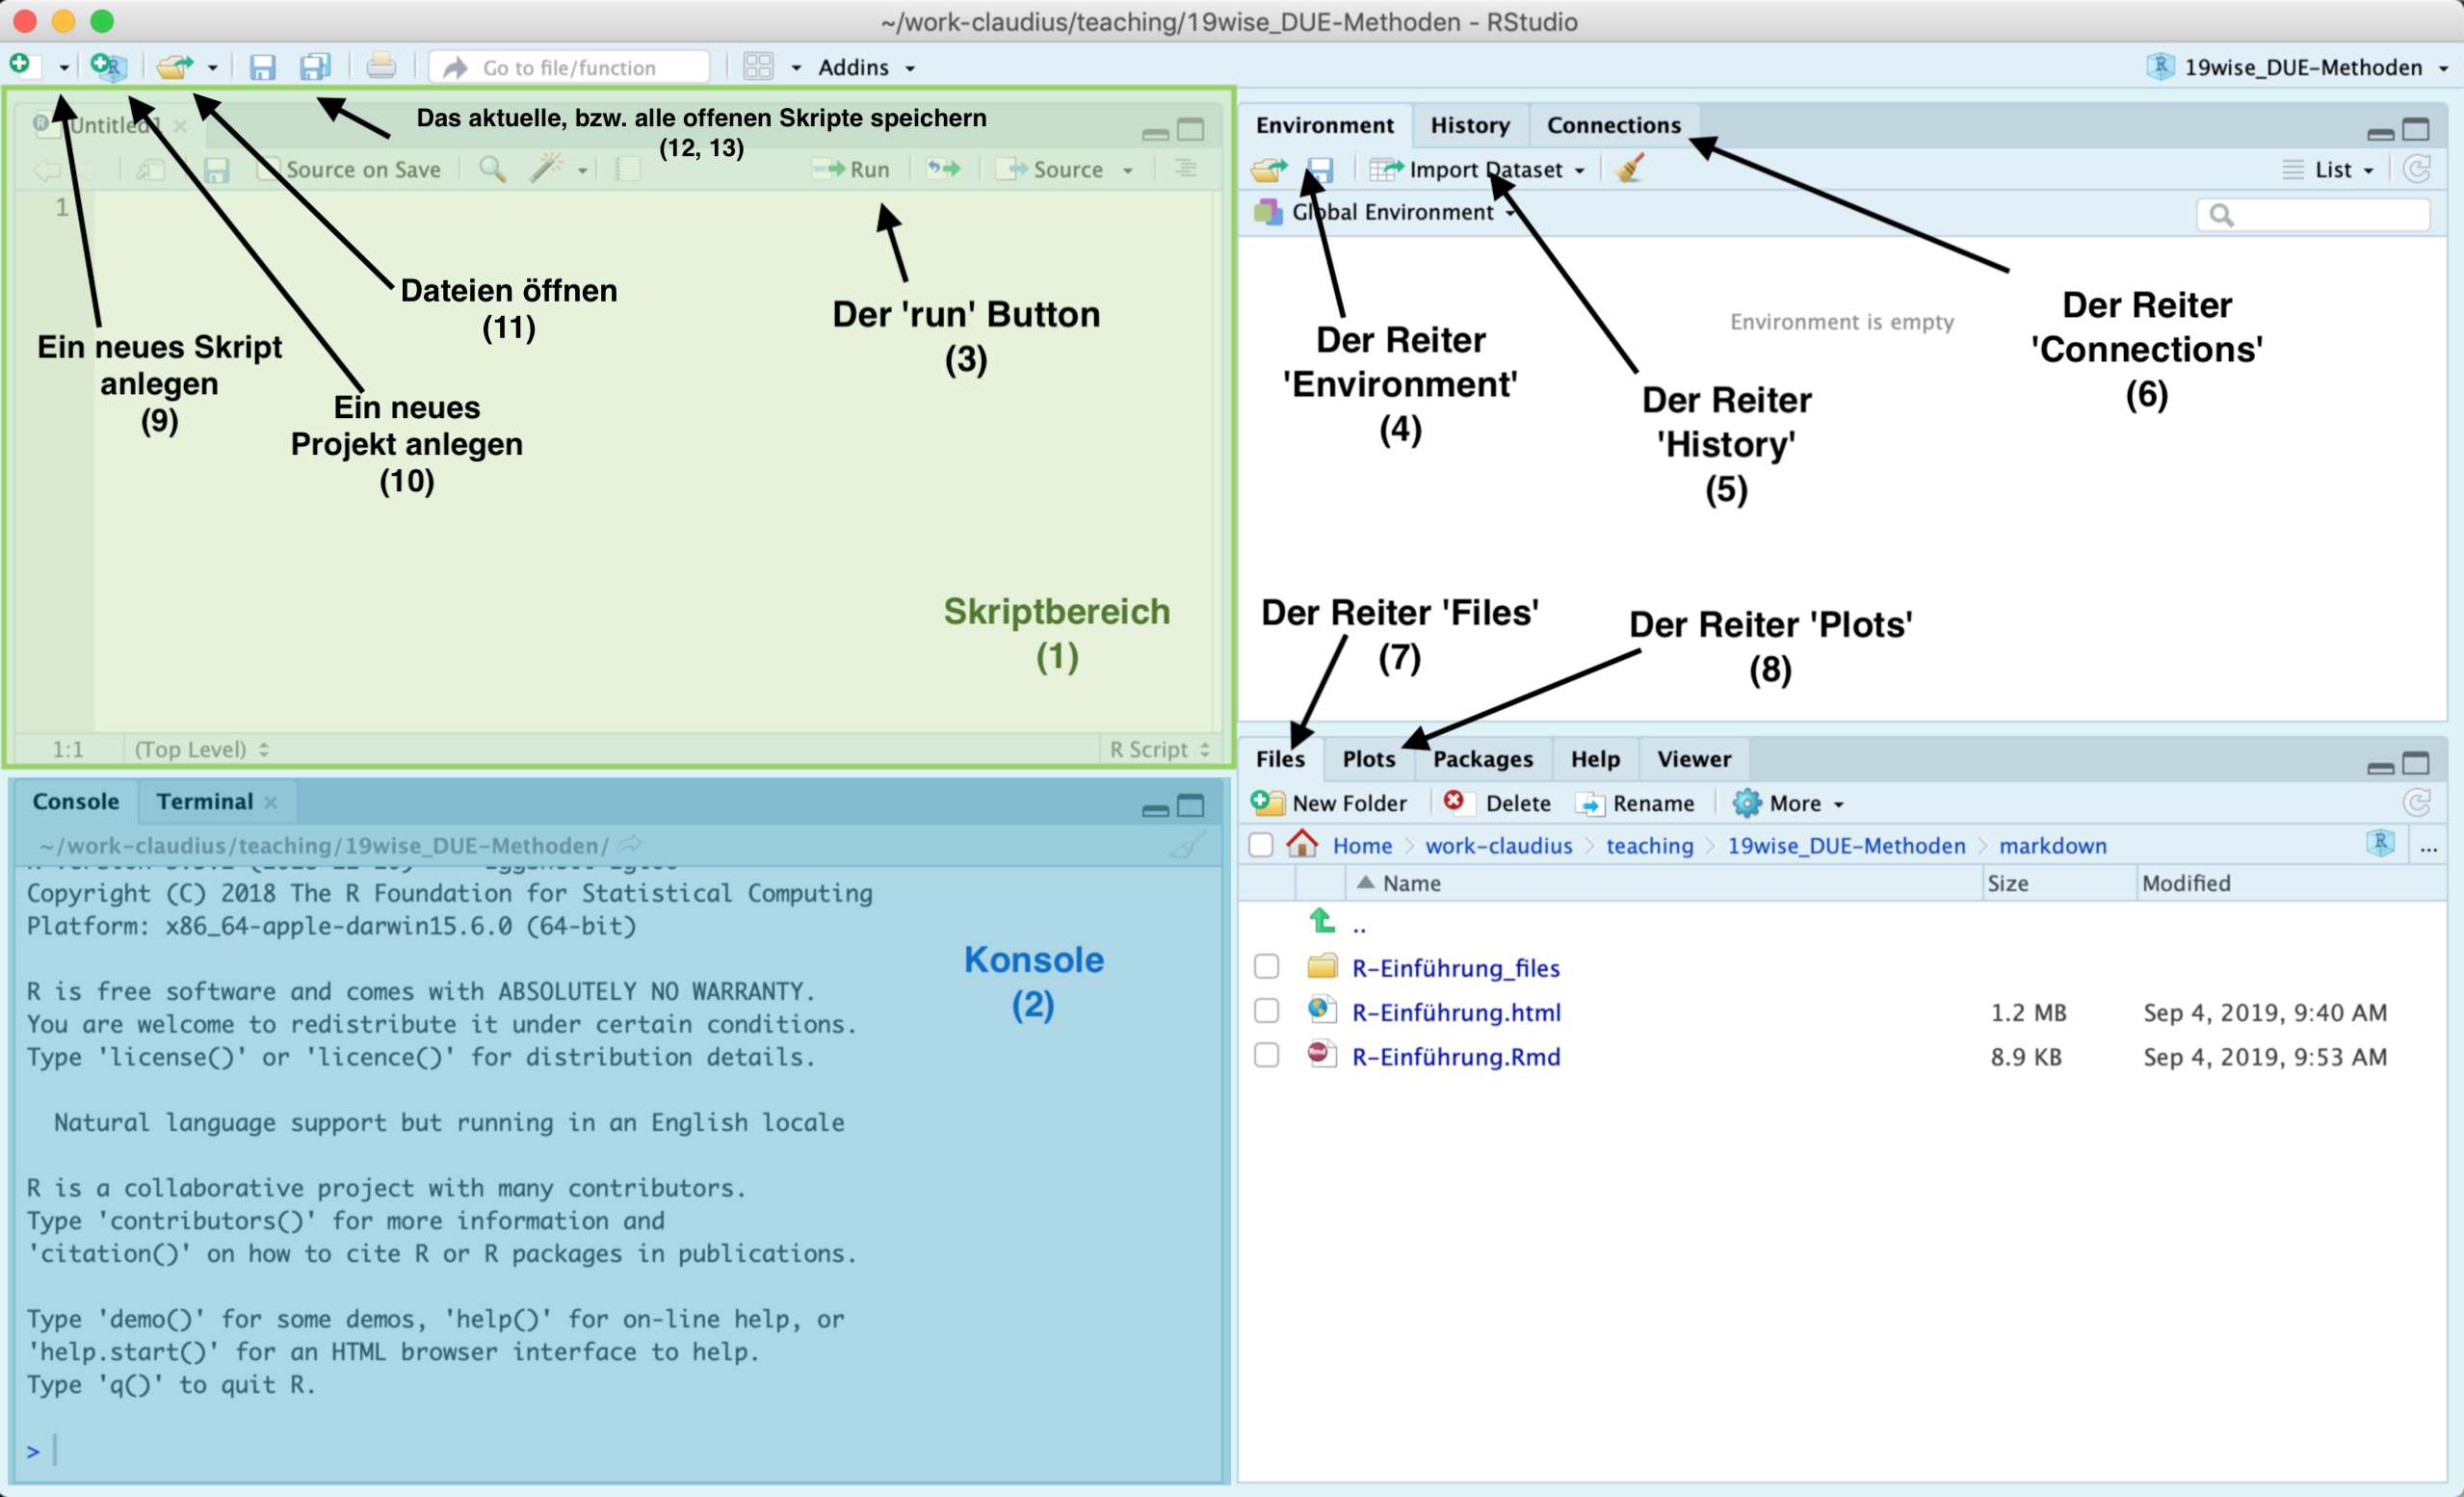
\includegraphics[width=1\linewidth]{figures/r-studio-light-marked} \end{center}

\begin{itemize}
\item
  Der \textbf{Skriptbereich} (1) ist ein Texteditor wie Notepad - nur
  mit zusätzlichen Features wie Syntax Highlighting für R, sodass es uns
  leichter fällt R Code zu schreiben. Hier werden wir unsere Skripte
  verfassen.
\item
  Die \textbf{Konsole} (2) erlaubt es uns über R direkt mit unserem
  Computer zu interagieren. R ist eine Programmiersprache. Das bedeutet,
  wenn wir den Regeln der Sprache folgen und uns in einer für den
  Computer verständlicher Art und Weise ausdrücken, versteht der
  Computer was wir von ihm wollen und führt unsere Befehle aus. Wenn wir
  in die Konsole z.B. \texttt{2+2} eingeben, dann ist das valider R
  code. Wenn wir dann Enter drücken versteht der Computer unseren Befehl
  und führt die Berechnung aus. Die Konsole ist sehr praktisch um den
  Effekt von R Code direkt zu beobachten. Wenn wir etwas in der Console
  ausführen wollen, das wir vorher im \textbf{Skriptbereich} geschrieben
  haben, können wir den Text markieren und dann auf den Button
  \texttt{Run} (3) drücken: dann kopiert R Studio den Code in die
  Konsole und führt ihn aus.
\item
  Für den Bereich oben rechts haben wir in der Standardkonfiguration von
  R Studio drei Optionen, die wir durch Klicken auf die Reiter auswählen
  können. Der Reiter \textbf{Environment} (4) zeigt uns alle bisher
  definierten Objekte an (mehr dazu später). Der Reiter \textbf{History}
  (5) zeigt an, welchen Code wir in der Vergangenheit ausgeführt haben.
  Der Reiter \textbf{Connections} (6) braucht uns aktuell nicht zu
  interessieren.
\item
  Auch für den Bereich unten rechts haben wir mehrere Optionen: Der
  Bereich \textbf{Files} (7) zeigt uns unser Arbeitsverzeichnis mit
  allen Ordnern und Dateien an. Das ist das gleiche, was wir auch über
  den File Explorer unserer Betriebssystems sehen würden. Der Bereich
  \textbf{Plots} (8) zeigt uns eine Vorschau der Abbildungen, die wir
  durch unseren Code produzieren. Die anderen Bereiche brauchen uns
  aktuell noch nicht zu interessieren.
\item
  Wenn wir ein neues R Skript erstellen wollen, können wir das über den
  Button \textbf{Neu} (9) erledigen. Wir klicken darauf und wählen die
  Option `R Skript'. Mit den alternativen Dateiformaten brauchen wir uns
  aktuell nicht beschäftigen.
\item
  Der Botton \textbf{Neues Projekt anlegen} (10) erstellt eine neues R
  Studio Projekt - mehr dazu in Kürze.
\item
  Der Button \textbf{Öffnen} (11) öffnet Dateien im Skriptbereich.
\item
  Die beiden Buttons \textbf{Speichern} (12) und \textbf{Alles
  speichern} (13) speichern das aktuelle, bzw. alle im Skriptbereich
  geöffnenten Dateien.
\end{itemize}

Die restlichen Buttons und Fenster in R Studio werden wir im Laufe der
Zeit kennenlernen.

Es macht Sinn, sich einmal die möglichen Einstellungsmöglichkeiten für R
Studio anzuschauen und ggf. eine andere Darstellungsversion zu wählen.

\section{Einrichtung eines R
Projekts}\label{einrichtung-eines-r-projekts}

Im folgenden werden wir lernen wie man ein neues R Projekt anlegt, R
Code schreiben und ausführen kann.

Wann immer wir ein neues Programmierprojekt starten, sollten wir dafür
einen eigenen Ordner anlegen und ein so genannten `R Studio Projekt'
erstellen. Das hilft uns den Überblick über unsere Arbeit zu behalten,
und macht es einfach Code untereinander auszutauschen.

Ein Programmierprojekt kann ein Projekt für eine Hausarbeit sein, die
Mitschriften für eine Vorlesungseinheit, oder einfach der Versuch ein
bestimmtes Problem zu lösen, z.B. einen Datensatz zu visualisieren.

Die Schritte zur Erstellung eines solchen Projekts sind immer die
gleichen:

\begin{enumerate}
\def\labelenumi{\arabic{enumi}.}
\tightlist
\item
  Einen Ordner für das Projekt anlegen.
\item
  Ein R-Studio Projekt in diesem Ordner erstellen.
\item
  Relevante Unterordner anlegen.
\end{enumerate}

Wir beschäftigen uns mit den Schritten gleich im Detail, müssen vorher
aber noch die folgenden Konzepte diskutieren: (1) das Konzept eines
\emph{Arbeitsverzeichnisses} (\emph{working directory}) und (2) die
Unterscheidnug zwischen \emph{absoluten} und \emph{relativen} Pfaden.

\subsection{Arbeitsverzeichnisse und
Pfade}\label{arbeitsverzeichnisse-und-pfade}

Das \textbf{Arbeitsverzeichnis} ist ein Ordner auf dem Computer, in dem
R standardmäßig sämtlichen Output speichert und von dem aus es auf
Datensätze und anderen Input zugreift. Wenn wir mit Projekten arbeiten
ist das Arbeitsverzeichnis der Ordner, in dem das R-Projektfile abgelegt
ist, ansonsten ist es euer Benutzerverzeichnis. Wir können uns das
Arbeitsverzeichnis mit der Funktion \texttt{getwd()} anzeigen lassen. In
meinem Fall ist das Arbeitsverzeichnis das folgende:

\begin{verbatim}
#> [1] "/Users/claudius/work-claudius/general/paper-projects/packages/SocioEconMethodsR"
\end{verbatim}

Wenn ich R nun sagen würde ein File unter dem Namen \texttt{test.pdf}
speichern, würde es am folgenden Ort gespeichert werden:

\begin{verbatim}
#> [1] "/Users/claudius/work-claudius/general/paper-projects/packages/SocioEconMethodsR/test.pdf"
\end{verbatim}

R geht in einem solchen Fall immer vom Arbeitsverzeichnis aus. Da wir im
vorliegenden Fall den Speicherort relativ zum Arbeitsverzeichnis
angegeben haben, sprechen wir hier von einem \textbf{relativen Pfad}.

Alternativ können wir den Speicherort auch als \textbf{absoluten Pfad}
angeben. In diesem Fall geben wir den kompletten Pfad, ausgehend vom
\href{https://de.wikipedia.org/wiki/Stammverzeichnis}{Root Verzeichnis}
des Computers, an. Wir würden R also \emph{explizit} auffordern, das
File an foldengem Ort zu speichern:

\begin{verbatim}
#> [1] "/Users/claudius/work-claudius/general/paper-projects/packages/SocioEconMethodsR/test.pdf"
\end{verbatim}

Wir werden hier \textbf{immer} relative Pfade verwenden. Relative Pfade
sind fast immer die bessere Variante, da es uns erlaubt den gleichen
Code auf verschiedenen Computern zu verwenden. Denn wiw man an den
absoluten Pfaden erkennen kann, sehen diese auf jedem Computer anders
aus und es ist dementsprechend schwierig, Code miteinander zu teilen.

Wir lernen mehr über dieses Thema wenn wir uns später mit Dateninput und
-output beschäftigen.

\subsection{Schritt 1: Projektordner
anlegen}\label{schritt-1-projektordner-anlegen}

Zuerst müssen Sie sich für einen Ordner auf Ihrem Computer entscheiden,
in dem alle Daten, die mit ihrem Projekt zu tun haben, also Daten,
Skripte, Abbildungen, etc. gespeichert werden sollen und diesen Ordner
gegebenenfalls neu erstellen. Es macht Sinn, einen solchen Ordner mit
einem informativen Namen ohne Leer- und Sonderzeichen zu versehen, z.B.
\texttt{SoSe19-Methodenkurs}.

Dieser Schritt kann theoretisch auch gemeinsam mit Schritt 2 erfolgen.

\subsection{Schritt 2: Ein R-Studio Projekt im Projektordner
erstellen}\label{schritt-2-ein-r-studio-projekt-im-projektordner-erstellen}

Wir möchten nun R Studio mitteilen den in Schritt 1 erstellten Ordner
als R Projekt zu behandeln. Damit wird nicht nur dieses Ordner als
Root-Verzeichnis festgelegt, man kann auch die Arbeitshistorie eines
Projekts leich wiederherstellen und es ist einfacher, das Projekt auf
verschiedenen Computern zu bearbeiten.

Um ein neues Projekt zu erstellen klicken Sie in R Studio auf den Button
\texttt{Neues\ Projekt} (Nr. 10 in der obigen Abbildung) und Sie sollten
folgendes Fenster sehen:

\begin{center}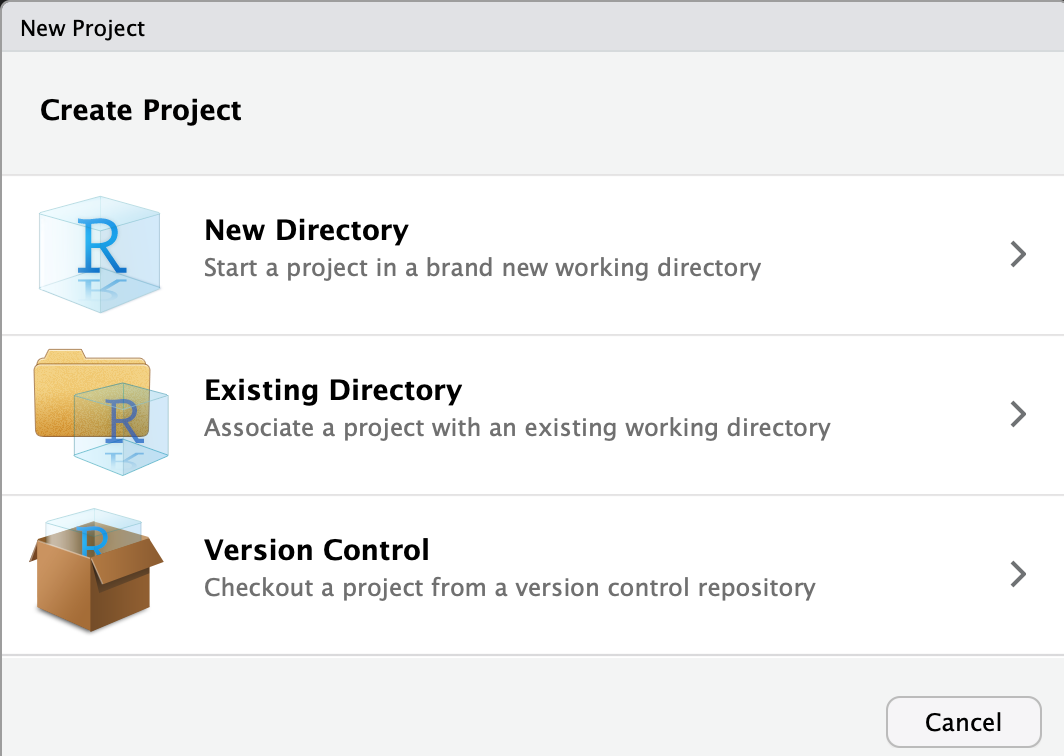
\includegraphics[width=0.6\linewidth]{figures/r-studio-new-project} \end{center}

Falls Sie in Schritt 1 den Projektordner bereits erstellt haben wählen
Sie hier \texttt{Existing\ Directory}, ansonsten erstellen Sie einen
neuen Projektordner gleich mit dem Projektfile mit indem Sie
\texttt{New\ Directory} auswählen.

Falls Sie \texttt{Existing\ Directory} gewählt haben, wählen Sie in
folgendem Fenster einfach den vorher erstellten Ordner aus und klickt
auf \texttt{Create\ Project}.

\begin{center}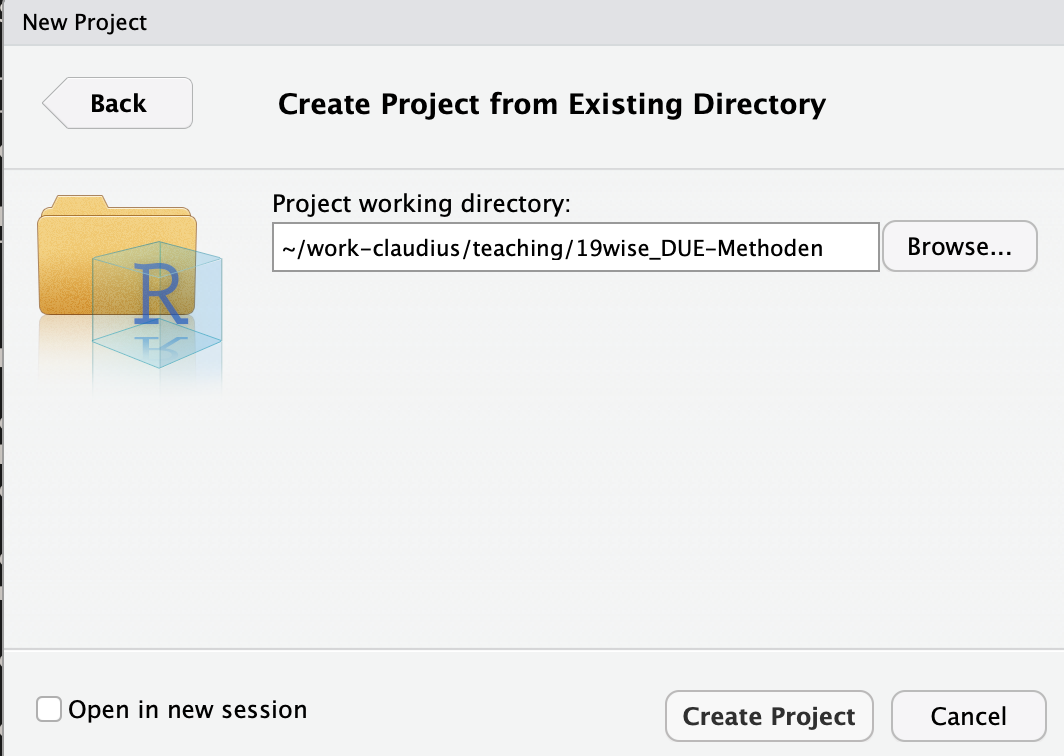
\includegraphics[width=0.6\linewidth]{figures/r-studio-new-project-exis-dir} \end{center}

Falls Sie \texttt{New\ Directory} gewählt habt landen Sie auf folgendem
Fenster:

\begin{center}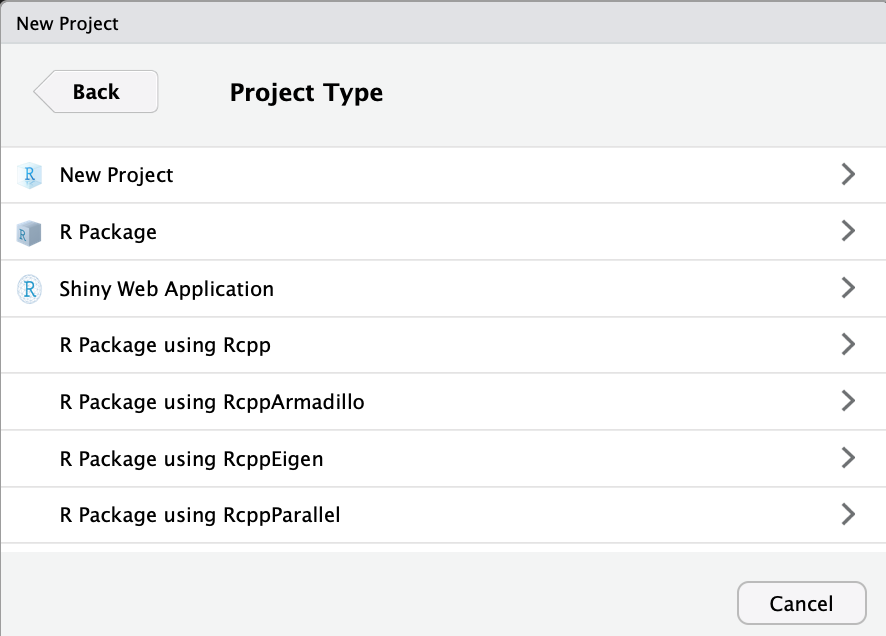
\includegraphics[width=0.6\linewidth]{figures/r-studio-new-project-new-dir} \end{center}

Hier wählen Sie \texttt{New\ Project} aus, geben dem Projekt in
folgenden Fenster einen Namen (das wird der Name des Projektordners
sein), wählen den Speicherort für den Ordner aus und klicken auf
\texttt{Create\ Project}.

In beiden Fällen wurde nun ein Ordner erstellt, in dem sich ein File
\texttt{*.Rproj} befindet. Damit ist die formale Erstellung eines
Projekts abgeschlossen. Es empfiehlt sich jedoch dringend gleich eine
sinnvolle Unterordnerstruktur mit anzulegen.

\hypertarget{unterordner}{\subsection{Schritt 3: Relevante Unterordner
erstellen}\label{unterordner}}

Eine sinnvolle Unterordnerstruktur hilf (1) den Überblick über das
eigene Projekt nicht zu verlieren, (2) mit anderen über verschiedene
Computer hinweg zu kollaborieren und (3) Kollaborationsplattformen wie
Github zu verwenden und replizierbare und für andere nachvollziehbare
Forschungsarbeit zu betreiben.

Die folgende Ordnerstruktur ist eine Empfehlung. In manchen Projekten
werden Sie nicht alle hier vorgeschlagenen Unterordner brauchen, in
anderen bietet sich die Verwendung von mehr Unterordnern an.
Nichtsdestotrotz ist es ein guter Ausgangspunkt, den ich in den meisten
meiner Forschungsprojekte auch so verwende.

Insgesamt sollten die folgenden Ordner im Projektordner erstellt werden:

\begin{itemize}
\tightlist
\item
  Ein Ordner \texttt{data}, der alle Daten enthält, die im Rahmen des
  Projekts verwendet werden. Hier empfiehlt es sich zwei Unterordner
  anzulegen: Einen Ordner \texttt{raw}, der die Rohdaten enthält, so wie
  sie aus dem Internet runtergeladen wurden. Diese Rohdaten sollten
  \textbf{niemals} verändert werden, ansonsten wird Ihre Arbeit nicht
  vollständig replizierbar werden und es kommt ggf. zu irreparablen
  Schäden. Alle Veränderungen der Daten sollten durch Skripte
  dokumentiert werdenn, die die Rohdaten als Input, und einen
  modifizierten Datensatz als Output generieren. Dieser modifizierte
  Datensatz sollte dann im Unterordner \texttt{tidy} gespeichert werden.
\end{itemize}

\begin{quote}
Beispiel: Sie laden sich Daten zum BIP in Deutschland von Eurostat und
Daten zu Arbeitslosigkeit von AMECO herunter. Beiden Datensätze sollten
im Unterordner \texttt{data/raw} gespeichert werden. Mit einem Skript
lesen Sie beide Datensätze ein und erstellen den kombinierten Datensatz
\texttt{macro\_data.csv}, den Sie im Ordner \texttt{data/tidy} speichern
und für die weitere Analyse verwenden. Dadurch kann jede*r
nachvollziehen wie die von Ihnen verwendeten Daten sich aus den Rohdaten
ergeben haben und Ihre Arbeit bleibt komplett transparent.
\end{quote}

\begin{itemize}
\item
  Ein Ordner \texttt{R}, der alle R Skripte enthält, also alle
  Textdokumente, die R Code enthalten.
\item
  Ein Ordner \texttt{output}, in dem der Output ihrer Berechnungen, z.B.
  Tabellen oder Plots gespeichert werden können. Der Inhalt dieses
  Ordners sollte sich komplett mit den Inhalten der Ordner \texttt{data}
  und \texttt{R} replizieren lassen.
\item
  Ein Ordner \texttt{text}, in dem Sie Ihre Verschriftlichungen
  speichern, z.B. das eigentliche Forschungspapier, ihre Hausarbeit oder
  Ihre Vorlesungsmitschriften.
\item
  Einen Ordner \texttt{misc} in den Sie alles packen, was in keinen der
  anderen Ordner passt. Ein solcher Ordner ist wichtig und Sie sollten
  nicht zuordbare Dateien nie in den Projektordner als solchen
  speichern.
\end{itemize}

Wenn wir annehmen unser Projektordner heißt \texttt{2019-Methoden}
ergibt sich damit insgesamt folgende Ordner und Datenstruktur:

\begin{center}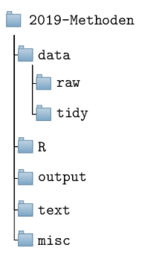
\includegraphics{figures/wd-structure} \end{center}

\section{Abschließende Bemerkungen}\label{abschlieende-bemerkungen}

Eine gute Ordnerstruktur ist nicht nur absolut essenziell um selbst
einen Überblick über seine Forschungsprojekte zu behalten, sondern auch
wenn man mit anderen Menschen kollaborieren möchte. In einem solchen
Fall sollte man auf jeden Fall eine Versionskontrolle wie Git und GitHub
verwenden. Wir werden uns damit im nächsten Semester genauer
beschäftigen, aber Sie werden merken, dass die Kollaboration durch eine
gut durchdachte Ordnerstruktur massiv erleichtert wird.

\chapter{Erste Schritte in R}\label{basics}

Nach diesen (wichtigen) Vorbereitungsschritten wollen wir nun mit dem
eigentlichen Programmieren anfangen. Zu diesem Zweck müssen wir uns mit
der Syntax von R vertraut machen, also mit den Regeln, denen wir folgen
müssen, wenn wir Code schreiben, damit der Computer versteht, was wir
ihm eigentlich in R sagen wollen.

\section{Befehle in R an den Computer
übermitteln}\label{befehle-in-r-an-den-computer-ubermitteln}

Grundsätzlich können wir über R Studio auf zwei Arten mit dem Computer
``kommunizieren'': über die Konsole direkt, oder indem wir im
Skriptbereich ein Skript schreiben und dies dann ausführen.

Als Beispiel für die erste Möglichkeit wollen wir mit Hilfe von R die
Zahlen \texttt{2} und \texttt{5} miteinander addieren. Zu diesem Zweck
können wir einfach \texttt{2\ +\ 2} in die Konsole eingeben, und den
Befehl mit `Enter' an den Computer senden. Da es sich beim Ausdruck
\texttt{2\ +\ 3} um korrekten R Code handelt, `versteht' der Computer
was wir von ihm wollen und gibt uns das entsprechende Ergebnis aus:

\begin{Shaded}
\begin{Highlighting}[]
\DecValTok{2} \OperatorTok{+}\StringTok{ }\DecValTok{3}
\end{Highlighting}
\end{Shaded}

\begin{verbatim}
#> [1] 5
\end{verbatim}

Auf diese Art und Weise könne wir R als einfachen Taschenrechner
verwenden, denn für alle einfachen mathematischen Operationen können wir
bestimmte Symbole als Operatoren verwenden. An dieser Stelle sei noch
darauf hingewiesen, dass das Symbol \texttt{\#} in R einen Kommentar
einleitet, das heißt alles was in einer Zeile nach \texttt{\#} steht
wird vom Computer ignoriert und man kann sich einfach Notizen in seinem
Code machen.

\begin{Shaded}
\begin{Highlighting}[]
\DecValTok{2} \OperatorTok{+}\StringTok{ }\DecValTok{2}  \CommentTok{# Addition}
\end{Highlighting}
\end{Shaded}

\begin{verbatim}
#> [1] 4
\end{verbatim}

\begin{Shaded}
\begin{Highlighting}[]
\DecValTok{2}\OperatorTok{/}\DecValTok{2}  \CommentTok{# Division}
\end{Highlighting}
\end{Shaded}

\begin{verbatim}
#> [1] 1
\end{verbatim}

\begin{Shaded}
\begin{Highlighting}[]
\DecValTok{4} \OperatorTok{*}\StringTok{ }\DecValTok{2}  \CommentTok{# Multiplikation}
\end{Highlighting}
\end{Shaded}

\begin{verbatim}
#> [1] 8
\end{verbatim}

\begin{Shaded}
\begin{Highlighting}[]
\DecValTok{3}\OperatorTok{^}\DecValTok{2}  \CommentTok{# Potenzierung}
\end{Highlighting}
\end{Shaded}

\begin{verbatim}
#> [1] 9
\end{verbatim}

Alternativ können wir die Befehle in einem Skript aufschreiben, und
dieses Skript dann ausführen. Während die Interaktion über die Konsole
sinnvoll ist um die Effekte bestimmter Befehle auszuprobieren, bietet
sich die Verwendung von Skripten an, wenn wir mit den Befehlen später
weiter arbeiten wollen, oder sie anderen Menschen zugänglich zu machen.
Den das Skript können wir als Datei auf unserem Computer speichern,
vorzugsweise im Unterordner \texttt{R} unseres R-Projekts (siehe
Abschnitt \protect\hyperlink{unterordner}{Relevante Unterordner
erstellen}), und dann später weiterverwenden.

Die Berechnungen, die wir bisland durchgeführt haben sind
zugegebenermaßen nicht sonderlich spannend. Um fortgeschrittene
Operationen in R durchführen und verstehen zu können müssen wir uns
zunächst mit den Konzepten von \textbf{Objekten}, \textbf{Funktionen}
und \textbf{Zuweisungen} beschäftigen.

\section{Objekte, Funktionen und
Zuweisungen}\label{objekte-funktionen-und-zuweisungen}

\begin{quote}
To understand computations in R, two slogans are helpful: Everything
that exists is an object. Everything that happens is a function call.
---John Chambers
\end{quote}

Mit der Aussage `Alles in R ist ein Objekt' ist gemeint, dass jede Zahl,
jede Funktion, oder jeder Buchstabe in R ein Objekt ist, das irgendwo
auf dem Speicher Ihres Rechners abgespeichert ist.

In der Berechnung \texttt{2\ +\ 3} ist die Zahl \texttt{2} genauso ein
Objekt wie die Zahl \texttt{3} und die Additionsfunktion, die durch den
Operator \texttt{+} aufgerufen wird.

Mit der Aussage `Alles was in R passiert ist ein Funktionsaufruf' ist
gemeint, dass wenn wir R eine Berechnung durchführen lassen, tun wir
dies indem wir eine Funktion aufrufen.

\textbf{Funktionen} sind Algorithmen, die bestimmte Routinen auf einen
\emph{Input} anwenden und dabei einen \emph{Output} produzieren. Die
Additionsfunktion, die wir in der Berechnung \texttt{2\ +\ 3} aufgerufen
haben hat als Input die beiden Zahlen \texttt{2} und \texttt{3}
aufgenommen, hat auf sie die Routine der Addition angewandt und als
Output die Zahl \texttt{5} ausgegeben. Der Output \texttt{5} ist dabei
in R genauso ein Objekt wie die Inputs \texttt{2} und \texttt{3}, sowie
die Funktion \texttt{+}.

Ein `Problem' ist, dass R im vorliegenden Falle den Output der
Berechnung zwar ausgibt, wir danach aber keinen Zugriff darauf mehr
haben:

\begin{Shaded}
\begin{Highlighting}[]
\DecValTok{2} \OperatorTok{+}\StringTok{ }\DecValTok{3}
\end{Highlighting}
\end{Shaded}

\begin{verbatim}
#> [1] 5
\end{verbatim}

Falls wir den Output weiterverwenden wollen, macht es Sinn, dem Output
Objekt einen Namen zu geben, damit wir später wieder darauf zugreifen
können. Der Prozess einem Objekt einen Namen zu Geben wird
\textbf{Zuweisung} oder \textbf{Assignment} genannt und durch die
Funktion \texttt{assign} vorgenommen:

\begin{Shaded}
\begin{Highlighting}[]
\KeywordTok{assign}\NormalTok{(}\StringTok{"zwischenergebnis"}\NormalTok{, }\DecValTok{2} \OperatorTok{+}\StringTok{ }\DecValTok{3}\NormalTok{)}
\end{Highlighting}
\end{Shaded}

Wir können nun das Ergebnis der Berechnung \texttt{2\ +\ 3} aufrufen,
indem wir in R den Namen des Output Objekts eingeben:

\begin{Shaded}
\begin{Highlighting}[]
\NormalTok{zwischenergebnis}
\end{Highlighting}
\end{Shaded}

\begin{verbatim}
#> [1] 5
\end{verbatim}

Da Zuweisungen so eine große Rolle spielen und sehr häufig vorkommen
gibt es auch für die Funktion \texttt{assign} eine Kurzschreibweise,
nämlich \texttt{\textless{}-}. Entsprechend sind die folgenden beiden
Befehle äquivalent:

\begin{Shaded}
\begin{Highlighting}[]
\KeywordTok{assign}\NormalTok{(}\StringTok{"zwischenergebnis"}\NormalTok{, }\DecValTok{2} \OperatorTok{+}\StringTok{ }\DecValTok{3}\NormalTok{)}
\NormalTok{zwischenergebnis <-}\StringTok{ }\DecValTok{2} \OperatorTok{+}\StringTok{ }\DecValTok{3}
\end{Highlighting}
\end{Shaded}

Entsprechend werden wir Zuweisungen immer mit dem \texttt{\textless{}-}
Operator durchführen. \footnote{Theoretisch kann \texttt{\textless{}-}
  auch andersherum verwendet werden:
  \texttt{2\ +\ 3\ -\textgreater{}\ zwischenergebnis}. Das mag zwar auf
  den ersten Blick intuitiver erscheinen, da das aus \texttt{2\ +\ 3}
  resultierende Objekt den Namen \texttt{zwischenergebnis} bekommt, also
  immer erst das Objekt erstellt wird und dann der Name zugewiesen wird,
  es führt jedoch zu deutlich weniger lesbarem Code und sollte daher nie
  verwendet werden. Ebensoweinig sollten Zuweisungen durch den
  \texttt{=} Operatur vorgenommen werden, auch wenn es im Fall
  \texttt{zwischenergebnis\ =\ 2\ +\ 3} funktionieren würde.}

Wir können in R nicht beliebig Namen vergeben. Gültige (also:
syntaktisch korrekte) Namen \ldots{}

\begin{itemize}
\tightlist
\item
  enthalten nur Buchstaben, Zahlen und die Symbole \texttt{.} und
  \texttt{\_}
\item
  fangen nicht mit \texttt{.} oder einer Zahl an!
\end{itemize}

Zudem gibt es einige Wörter, die schlicht nicht als Name verwendet
werden dürgen, z.B. \texttt{function}, \texttt{TRUE}, oder \texttt{if}.
Die gesamte Liste verbotener Worte kann mit dem Befehl
\texttt{?Reserved} ausgegeben werden.

Wenn man einen Namen vergeben möchte, der nicht mit den gerade
formulierten Regeln kompatibel ist, gibt R eine Fehlermeldung aus:

\begin{Shaded}
\begin{Highlighting}[]
\OtherTok{TRUE}\NormalTok{ <-}\StringTok{ }\DecValTok{5}
\end{Highlighting}
\end{Shaded}

\begin{verbatim}
#> Error in TRUE <- 5: invalid (do_set) left-hand side to assignment
\end{verbatim}

Zudem sollte man folgendes beachten:

\begin{itemize}
\tightlist
\item
  Namen sollten kurz und informativ sein; entsprechen ist
  \texttt{sample\_mean} ein guter Name, \texttt{shit15\_2} dagegen eher
  weniger
\item
  Man sollte \textbf{nie Umlaute in Namen verwenden}
\item
  R ist \emph{case sensitive}, d.h. \texttt{mean\_value} ist ein anderer
  Name als \texttt{Mean\_Value}
\item
  Auch wenn möglich, sollte man nie von R bereit gestellte Funktionen
  überschreiben. Eine Zuweisung wie \texttt{assign\ \textless{}-\ 2} ist
  zwar möglich, führt in der Regel aber zu großem Unglück, weil man
  nicht mehr ganz einfach auf die zugrundeliegende Funktion
  zurückgreifen kann.
\end{itemize}

\begin{quote}
\textbf{Hinweis}: Alle aktuellen Namenszuweisungen sind im Bereich
\texttt{Environment} in R Studio (Nr. 4 in der Abbildung oben)
aufgelistet und können durch die Funktion \texttt{ls()} angezeigt
werden.
\end{quote}

\begin{quote}
\textbf{Hinweis}: Ein Objekt kann mehrere Namen haben, aber kein Name
kann zu mehreren Objekten zeigen, da im Zweifel eine neue Zuweisung die
alte Zuweisung überschreibt:
\end{quote}

\begin{Shaded}
\begin{Highlighting}[]
\NormalTok{x <-}\StringTok{ }\DecValTok{2}
\NormalTok{y <-}\StringTok{ }\DecValTok{2}  \CommentTok{# Das Objekt 2 hat nun zwei Namen}
\KeywordTok{print}\NormalTok{(x)}
\end{Highlighting}
\end{Shaded}

\begin{verbatim}
#> [1] 2
\end{verbatim}

\begin{Shaded}
\begin{Highlighting}[]
\KeywordTok{print}\NormalTok{(y)}
\end{Highlighting}
\end{Shaded}

\begin{verbatim}
#> [1] 2
\end{verbatim}

\begin{Shaded}
\begin{Highlighting}[]
\NormalTok{x <-}\StringTok{ }\DecValTok{4}  \CommentTok{# Der Name 'x' zeigt nun zum Objekt '4', nicht mehr zu '2'}
\KeywordTok{print}\NormalTok{(x)}
\end{Highlighting}
\end{Shaded}

\begin{verbatim}
#> [1] 4
\end{verbatim}

\begin{quote}
\textbf{Hinweis}: Wie Sie vielleicht bereits bemerkt haben wird nach
einer Zuweisung kein Wert sichtbar ausgegeben:
\end{quote}

\begin{Shaded}
\begin{Highlighting}[]
\DecValTok{2} \OperatorTok{+}\StringTok{ }\DecValTok{2}  \CommentTok{# Keine Zuweisung, R gibt das Ergebnis in der Konsole aus}
\end{Highlighting}
\end{Shaded}

\begin{verbatim}
#> [1] 4
\end{verbatim}

\begin{Shaded}
\begin{Highlighting}[]
\NormalTok{x <-}\StringTok{ }\DecValTok{2} \OperatorTok{+}\StringTok{ }\DecValTok{2}  \CommentTok{# Zuweisung, R gibt das Ergebnis in der Konsole nicht aus}
\end{Highlighting}
\end{Shaded}

\section{Zusammenfassung}\label{zusammenfassung}

\begin{itemize}
\tightlist
\item
  Wir können Befehle in R Studio an den Computer übermitteln indem wir
  (a) den R Code in die Konsole schreiben und Enter drücken oder (b) den
  Code in ein Skript schreiben und dann ausführen
\item
  Alles was in R \emph{existiert} ist ein Objekt, alles was in R
  \emph{passiert} ist ein Funktionsaufruf
\item
  Wir können einem Objekt mit Hilfe von \texttt{\textless{}-} einen
  Namen geben und dann später wieder aufrufen. Den Prozess der
  Namensgebung nennen wir \textbf{Assignment} und wir können uns alle
  aktuell von uns vergebenen Namen mit der Funktion \texttt{ls()}
  anzeigen lassen.
\item
  Eine Funktion ist ein Objekt, das auf einen Input eine bestimmte
  Routine anwendet und einen Output produziert
\end{itemize}

An dieser Stelle sei noch auf die Hilfefunktion \texttt{help()}
hingewiesen. Falls Sie Informationen über ein Objekt bekommen wollen
können Sie so weitere Informationen bekommen. Wenn Sie z.B. genauere
Informationen über die Verwendung der Funktion \texttt{assign} erhalten
wollen, können Sie Folgendes eingeben:

\begin{Shaded}
\begin{Highlighting}[]
\KeywordTok{help}\NormalTok{(assign)}
\end{Highlighting}
\end{Shaded}

\section{Grundlegende Objeke in R}\label{grundlegende-objeke-in-r}

Wir haben bereits gelernt, dass alles was in R existiert ein Objekt ist.
Wir haben aber auch schon gelernt, dass es unterschiedliche Typen von
Objekten gibt: Zahlen, wie \texttt{2} oder \texttt{3} und Funktionen wie
\texttt{assign}.\footnote{Wie wir unten lernen werden sind \texttt{2}
  und \texttt{3} in erster Linie keine Zahlen, sondern Vektoren der
  Länge 1, und gelten erst in nächster Instanz als `Zahl' (genauer:
  `double').} Tatsächlich gibt es noch viel mehr Arten von Objekten. Ein
gutes Verständnis der Objektarten ist Grundvoraussetzung später
anspruchsvolle Programmieraufgaben zu lösen. Daher wollen wir uns im
Folgenden mit den wichtigsten Objektarten in R auseinandersetzen.

\subsection{Funktionen}\label{funktionen}

Wie oben bereits kurz erwähnt handelt es sich bei Funktionen um
Algorithmen, die bestimmte Routinen auf einen \emph{Input} anwenden und
dabei einen \emph{Output} produzieren.

Die Funktion \texttt{log()} zum Beispiel nimmt als Input eine Zahl und
gibt als Output den Logarithmus dieser Zahl aus:

\begin{Shaded}
\begin{Highlighting}[]
\KeywordTok{log}\NormalTok{(}\DecValTok{2}\NormalTok{)}
\end{Highlighting}
\end{Shaded}

\begin{verbatim}
#> [1] 0.6931472
\end{verbatim}

\textbf{Eine Funktion aufrufen}

In R gibt es prinzipiell vier verschiedene Arten Funktionen aufzurufen.
Nur zwei davon sind allerdings aktuell für uns relevant.

Die bei weitem wichtigste Variante ist die so genannte
\emph{Prefix-Form}. Dies ist die Form, die wir bei der überwältigenden
Anzahl von Funktionen verwenden werden. Wir schreiben hier zunächst den
Namen der Funktion (im Folgenden Beispiel \texttt{assign}), dann in
Klammern und mit Kommata getrennt die Argumente der Funktion (hier der
Name \texttt{test} und die Zahl \texttt{2}):

\begin{Shaded}
\begin{Highlighting}[]
\KeywordTok{assign}\NormalTok{(}\StringTok{"test"}\NormalTok{, }\DecValTok{2}\NormalTok{)}
\end{Highlighting}
\end{Shaded}

Ein hin und wieder auftretende Form ist die so genannte
\emph{Infix-Form}. Hier wird der Funktionsname zwischen die Argumente
geschrieben. Dies ist, wie wir oben bereits bemerkt haben, bei vielen
mathematischen Funktionen wie \texttt{+}, \texttt{-} oder \texttt{/} der
Fall. Streng genommen ist die die Infix-Form aber nur eine
\emph{Abkürzung}, denn jeder Funktionsaufruf in Infix-Form kann auch in
Prefix-Form geschrieben werden, wie folgendes Beispiel zeigt:

\begin{Shaded}
\begin{Highlighting}[]
\DecValTok{2} \OperatorTok{+}\StringTok{ }\DecValTok{3}
\end{Highlighting}
\end{Shaded}

\begin{verbatim}
#> [1] 5
\end{verbatim}

\begin{Shaded}
\begin{Highlighting}[]
\DecValTok{2} \OperatorTok{+}\StringTok{ }\DecValTok{3}
\end{Highlighting}
\end{Shaded}

\begin{verbatim}
#> [1] 5
\end{verbatim}

\textbf{Die Argumente einer Funktion}

Die Argumente einer Funktion stellen zum einen den \emph{Input} für die
in der Funktion implementierten Routine dar.

Die Funktion \texttt{sum} zum Beispiel nimmt als Argumente eine
beliebige Anzahl an Zahlen (ihr `Input') und berechnet die Summe dieser
Zahlen:

\begin{Shaded}
\begin{Highlighting}[]
\KeywordTok{sum}\NormalTok{(}\DecValTok{1}\NormalTok{, }\DecValTok{2}\NormalTok{, }\DecValTok{3}\NormalTok{, }\DecValTok{4}\NormalTok{)}
\end{Highlighting}
\end{Shaded}

\begin{verbatim}
#> [1] 10
\end{verbatim}

Darüber hinaus akzeptiert \texttt{sum()} noch ein \emph{optionales
Argument}, \texttt{na.rm}, welches entweder den Wert \texttt{TRUE} oder
\texttt{FALSE} annehmen kann. Wenn wir das Argument nicht explizit
spezifizieren nimmt es automatisch \texttt{FALSE} als den Standardwert
an.

Dieses optionale Argument ist kein klassischer Input, sondern
kontrolliert das genaue Verhalten der Funktion. Im Falle von
\texttt{sum()} werden fehlende Werte, so genannte \texttt{NA} (siehe
unten) ignoriert bevor die Summe der Inputs gebildet wird wenn
\texttt{na.rm} den Wert \texttt{TRUE} hat:

\begin{Shaded}
\begin{Highlighting}[]
\KeywordTok{sum}\NormalTok{(}\DecValTok{1}\NormalTok{, }\DecValTok{2}\NormalTok{, }\DecValTok{3}\NormalTok{, }\DecValTok{4}\NormalTok{, }\OtherTok{NA}\NormalTok{)}
\end{Highlighting}
\end{Shaded}

\begin{verbatim}
#> [1] NA
\end{verbatim}

\begin{Shaded}
\begin{Highlighting}[]
\KeywordTok{sum}\NormalTok{(}\DecValTok{1}\NormalTok{, }\DecValTok{2}\NormalTok{, }\DecValTok{3}\NormalTok{, }\DecValTok{4}\NormalTok{, }\OtherTok{NA}\NormalTok{, }\DataTypeTok{na.rm =} \OtherTok{TRUE}\NormalTok{)}
\end{Highlighting}
\end{Shaded}

\begin{verbatim}
#> [1] 10
\end{verbatim}

Wenn wir wissen wollen, welche Argumente eine Funktion akzeptiert ist es
immer eine gute Idee über die Funktion \texttt{help()} einen Blick in
die Dokumentation zu werfen!

Im Falle von \texttt{sum()} sehen wir hier sofort, dass die Funktion
neben den zu addierenden Zahlen ein optionales Argument \texttt{na.rm}
akzeptiert, welches den Standardwert \texttt{FALSE} annimmt.

\textbf{Eigene Funktionen definieren}

Sehr häufig möchten wir selbst Funktionen definieren. Das können wir mit
dem reservierten Keyword \texttt{function} machen. Als Beispiel wollen
wir eine Funktion \texttt{pythagoras} definieren, die als Argumente die
Seitenlängen der Katheten eines rechtwinkligen Dreiecks annimmt und über
den \href{https://de.wikipedia.org/wiki/Satz_des_Pythagoras}{Satz des
Pythagoras} die Länge der Hypothenuse bestimmt:

\begin{Shaded}
\begin{Highlighting}[]
\NormalTok{pythagoras <-}\StringTok{ }\ControlFlowTok{function}\NormalTok{(kathete_}\DecValTok{1}\NormalTok{, kathete_}\DecValTok{2}\NormalTok{) \{}
\NormalTok{    hypo_quadrat <-}\StringTok{ }\NormalTok{kathete_}\DecValTok{1}\OperatorTok{^}\DecValTok{2} \OperatorTok{+}\StringTok{ }\NormalTok{kathete_}\DecValTok{2}\OperatorTok{^}\DecValTok{2}
\NormalTok{    l_hypothenuse <-}\StringTok{ }\KeywordTok{sqrt}\NormalTok{(hypo_quadrat)  }\CommentTok{# sqrt() zieht die Quadratwurzel}
    \KeywordTok{return}\NormalTok{(l_hypothenuse)}
\NormalTok{\}}
\end{Highlighting}
\end{Shaded}

Wir definieren eine Funktion durch die Funktion \texttt{function()}. In
der Regel beginnen wir die Definition indem wir der zu erstellenden mit
einem Namen assoziieren (hier: `pythagoras') damit wir sie später auch
verwenden können.

Die Argumente für \texttt{function} sind dann die Argumente, welche die
zu definierende Funktion annehmen soll, in diesem Fall
\texttt{kathete\_1} und \texttt{kathete\_2}. Danach beginnen wir den
`function body', also den Code für die Routine, welche die Funktion
ausführen soll, mit einer geschweiften Klammer.

Innerhalb des \emph{function bodies} wird dann die entsprechende Routine
implementiert. Im vorliegenden Beispiel definieren wir zunächst die
Summe der Werte von \texttt{kathete\_1} und \texttt{kathete\_2} als ein
Zwischenergebnis, welches hier \texttt{hypo\_quadrat} genannt wird. Dies
ist der häufig unter \(c^2=a^2 + b^2\) bekannte Teil des Satz von
Pythagoras. Da wir an der `normalen' Länge der Hypothenuse interesssiert
sind, ziehen wir mit der Funktion \texttt{sqrt()} noch die Wurzel von
\texttt{hypo\_quadrat}, und geben dem resultierenden Objekt den Namen
\texttt{l\_hypothenuse}, welches in der letzten Zeile mit Hilfe des
Keywords \texttt{return} als der Wert definiert wird, den die Funktion
als Output ausgibt.\footnote{Das ist strikt genommen nicht notwendig,
  aber der Übersichtlichkeit werden wir immer \texttt{return} verwenden.
  Eine interessante Debatte darüber ob man \texttt{return} verwenden
  sollte oder nicht findet sich
  \href{https://stackoverflow.com/questions/11738823/explicitly-calling-return-in-a-function-or-not}{hier}.}

Am Ende der Routine kann man mit dem Keyword \texttt{return} explizit
machen welchen Wert die Funktion als Output ausgeben soll. Wenn wir die
Funktion nun aufrufen wird die oben definierte Routine ausgeführt:

\begin{Shaded}
\begin{Highlighting}[]
\KeywordTok{pythagoras}\NormalTok{(}\DecValTok{2}\NormalTok{, }\DecValTok{4}\NormalTok{)}
\end{Highlighting}
\end{Shaded}

\begin{verbatim}
#> [1] 4.472136
\end{verbatim}

Beachten Sie, dass alle Objet Namen, die innerhalb des \emph{function
bodies} verwendet werden gehen nach dem Funktionsaufruf
verloren:\footnote{Das liegt daran, dass Funktionen ihr eigenes
  \href{https://adv-r.hadley.nz/environments.html}{environment} haben.}
Deswegen kommt es im vorliegenden Falle zu einem Fehler, da
\texttt{hypo\_quadrat} nur innerhalb des \emph{function bodies}
existiert:

\begin{Shaded}
\begin{Highlighting}[]
\NormalTok{pythagoras <-}\StringTok{ }\ControlFlowTok{function}\NormalTok{(kathete_}\DecValTok{1}\NormalTok{, kathete_}\DecValTok{2}\NormalTok{) \{}
\NormalTok{    hypo_quadrat <-}\StringTok{ }\NormalTok{kathete_}\DecValTok{1}\OperatorTok{^}\DecValTok{2} \OperatorTok{+}\StringTok{ }\NormalTok{kathete_}\DecValTok{2}\OperatorTok{^}\DecValTok{2}
\NormalTok{    l_hypothenuse <-}\StringTok{ }\KeywordTok{sqrt}\NormalTok{(hypo_quadrat)  }\CommentTok{# sqrt() zieht die Quadratwurzel}
    \KeywordTok{return}\NormalTok{(l_hypothenuse)}
\NormalTok{\}}
\NormalTok{x <-}\StringTok{ }\KeywordTok{pythagoras}\NormalTok{(}\DecValTok{2}\NormalTok{, }\DecValTok{4}\NormalTok{)}
\NormalTok{hypo_quadrat}
\end{Highlighting}
\end{Shaded}

\begin{verbatim}
#> Error in eval(expr, envir, enclos): object 'hypo_quadrat' not found
\end{verbatim}

Es ist immer eine gute Idee, die selbst definierten Funktionen zu
dokumentieren - nicht nur wenn wir sie auch anderen zur Verfügung
stellen wollen, sondern auch damit wir selbst nach einer möglichen Pause
unseren Code noch gut verstehen können. Nichts ist frustrierender als
nach einer mehrwöchigen Pause viele Stunden investieren zu müssen, den
eigens programmierten Code zu entschlüsseln!

Die Dokumentation von Funktionen kann mit Hilfe von einfachen
Kommentaren erfolgen, ich empfehle jedoch sofort sich die
\href{https://r-pkgs.org/man.html\#man-functions}{hier beschriebenen
Konventionen} anzugewöhnen. In diesem Falle würde eine Dokumentation
unserer Funktion \texttt{pythagoras} folgendermaßen aussehen:

\begin{Shaded}
\begin{Highlighting}[]
\CommentTok{#' Berechne die Länge der Hypothenuse in einem rechtwinkligen Dreieck}
\CommentTok{#' }
\CommentTok{#' Diese Funktion nimmt als Argumente die Längen der beiden Katheten eines}
\CommentTok{#'  rechtwinkligen Dreiecks und berechnet daraus die Länge der Hypothenuse.}
\CommentTok{#' @param kathete_1 Die Länge der ersten Kathete}
\CommentTok{#' @param kathete_2 Die Länge der zweiten Kathete}
\CommentTok{#' @return Die Länge der Hypothenuse des durch a und b definierten }
\CommentTok{#'  rechtwinkligen Dreieckst}
\NormalTok{pythagoras <-}\StringTok{ }\ControlFlowTok{function}\NormalTok{(kathete_}\DecValTok{1}\NormalTok{, kathete_}\DecValTok{2}\NormalTok{) \{}
\NormalTok{    hypo_quadrat <-}\StringTok{ }\NormalTok{kathete_}\DecValTok{1}\OperatorTok{^}\DecValTok{2} \OperatorTok{+}\StringTok{ }\NormalTok{kathete_}\DecValTok{2}\OperatorTok{^}\DecValTok{2}
\NormalTok{    l_hypothenuse <-}\StringTok{ }\KeywordTok{sqrt}\NormalTok{(hypo_quadrat)  }\CommentTok{# sqrt() zieht die Quadratwurzel}
    \KeywordTok{return}\NormalTok{(l_hypothenuse)}
\NormalTok{\}}
\end{Highlighting}
\end{Shaded}

Die Dokumentation wird also direkt vor die Definition der Funktion
gesetzt. In der ersten Zeile gibt man der Funktion einen maximal
einzeiligen Titel, der nicht länger als 80 Zeichen sein sollte und die
Funktion prägnant beschreibt.

Dann, nach einer Lehrzeile wird genauer beschrieben was die Funktion
macht. Danach werden die Argumente der Funktion beschrieben. Für jedes
Argument beginnen wir die Reihe mit \texttt{@param}, gefolgt von dem
Namen des Arguments und dann einer kurzen Beschreibung.

Nach den Argumenten beschreiben wir noch kurz was der Output der
Funktion ist. Diese Zeile wird mit \texttt{@return} begonnen.

Die Dokumentation einer Funktion sollte also zumindest die Parameter und
die Art des Outputs erklären.

\textbf{Gründe für die Verwendung eigener Funktionen}

Eigene Funktionen zu definieren ist in der Praxis extrem hilfreich und
es ist empfehlenswert Routinen, die mehrere Male verwendet werden
grundsätzlich als Funktionen zu schreiben. Dafür gibt es mehrere Gründe:

\begin{enumerate}
\def\labelenumi{\arabic{enumi}.}
\tightlist
\item
  \textbf{Der Code wird kürzer und transparenter.} Zwar ist kurzer Code
  nicht notwendigerweise leichter zu verstehen als langer, aber
  Funktionen können besonders gut dokumentiert werden (am besten indem
  man den hier beschriebenen Konventionen folgt).
\item
  \textbf{Funktionen bieten Struktur.} Funktionen fassen in der Regel
  Ihre Vorstellung davon zusammen, wie ein bestimmtes Problem zu lösen
  ist. Da man sich diese Gedanken nicht ständig neu machen möchte ist es
  sinnvoll sie einmalig in einer Funktion zusammen zu fassen.
\item
  \textbf{Funktionen erleichtern Korrekturen.} Wenn Sie merken, dass Sie
  in der Implementierung einer Routine einen Fehler gemacht haben müssen
  Sie im besten Falle nur einmal die Definition der Funktion korrigieren
  - im schlimmsten Falle müssen sie in ihrem Code nach der Routine
  suchen und sie in jedem einzelnen Anwendungsfall erneut korrigieren.
\end{enumerate}

Es gibt noch viele weitere Gründe dafür, Funktionen häufig zu verwenden.
Viele hängen mit dem Entwicklerprinzip
\href{https://de.wikipedia.org/wiki/Don\%E2\%80\%99t_repeat_yourself}{DRY}
(``Don't Repeat Yourself'') zusammen.

\subsection{Vektoren}\label{vektoren}

Vektoren sind einer der wichtigsten Objektypen in R. Quasi alle Daten
mit denen wir in R arbeiten werden als Vektoren behandelt.

Was Vektoren angeht gibt es wiederum die wichtige \textbf{Unterscheidung
von atomaren Vektoren und Listen}. Beide bestehen ihrerseits aus
Objekten und sie unterscheiden sich dadurch, dass atomare Vektoren nur
aus Objekten des gleichen Typs bestehen können, Listen dagegen auch
Objekte unterschiedlichen Typs beinhalten können.

Entsprechend kann jeder atomare Vektor einem Typ zugeordnet werden, je
nachdem welchen Typ seine Bestandteile haben. Hier sind insbesondere
vier Typen relevant:

\begin{itemize}
\tightlist
\item
  \texttt{logical} (logische Werte): es gibt zwei logische Werte,
  \texttt{TRUE} und \texttt{FALSE}, welche auch mit \texttt{T} oder
  \texttt{F} abgekürzt werden können
\item
  \texttt{integer} (ganze Zahlen): das sollte im Prinzip selbsterklärend
  sein, allerding muss den ganzen Zahlen in R immer der Buchstabe
  \texttt{L} folgen, damit die Zahl tatsächlich als ganze Zahl
  interpretiert wird.\footnote{Diese auf den ersten Blick merkwürdige
    Syntax hat historische Gründe: als der integer Typ in die R
    Programmiersprache eingeführt wurde war er sehr stark an den Typ
    \texttt{long\ integer} in der Programmiersprache `C' angelehnt. In C
    wurde ein solcher `long integer' mit dem Suffix `l' oder `L'
    definiert, diese Regel wurde aus Kompatibilitätsgründen auch für R
    übernommen, jedoch nur mit `L', da man Angst hatte, dass `l' mit `i'
    verwechselt wird, was in R für die imaginäre Komponente komplexer
    Zahlen verwendet wird.} Beispiele sind \texttt{1L}, \texttt{400L}
  oder \texttt{10L}.\\
\item
  \texttt{double} (Dezimalzahlen): auch das sollte selbsterklärend sein;
  Beispiele wären \texttt{1.5}, \texttt{0.0}, oder \texttt{-500.32}.
\item
  Ganze Zahlen und Dezimalzahlen werden häufig unter der Kategorie
  \texttt{numeric} zusammengefasst. Dies ist in der Praxis aber quasi
  nie hilfreich und man sollte diese Kategorie möglichst nie verwenden.
\item
  Wörter (\texttt{character}): sie sind dadurch gekennzeichnet, dass sie
  auch Buchstaben enthalten können und am Anfang und Ende ein \texttt{"}
  haben. Beispiele hier wären \texttt{"Hallo"}, \texttt{"500"} oder
  \texttt{"1\_2\_Drei"}.
\item
  Es gibt noch zwei weitere besondere `Typen', die strikt gesehen keine
  atomaren Vektoren darstellen, allerdings in diesem Kontext schon
  häufig auftauchen: \texttt{NULL}, was strikt genommen ein eigener
  Datentyp ist und immer die Länge 0 hat, sowie \texttt{NA}, das einen
  fehlenden Wert darstellt
\end{itemize}

Hieraus ergibt sich folgende Aufteilung für Vektoren:

\begin{center}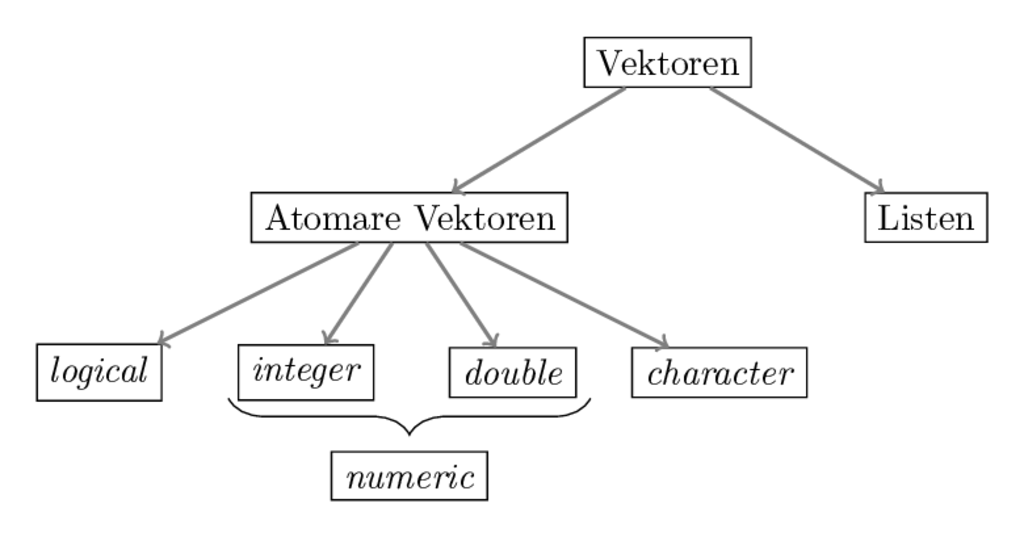
\includegraphics[width=0.8\linewidth]{figures/vector-classification} \end{center}

Wir werden nun die einzelnen Typen genauer betrachten. Vorher wollen wir
jedoch noch die Funktion \texttt{typeof} einführen. Sie hilft uns in der
Praxis den Typ eines Objekts herauszufinden. Dafür rufen wir einfach die
Funktion \texttt{typeof} mit dem zu untersuchenden Objekt oder dessen
Namen auf:

\begin{Shaded}
\begin{Highlighting}[]
\KeywordTok{typeof}\NormalTok{(2L)}
\end{Highlighting}
\end{Shaded}

\begin{verbatim}
#> [1] "integer"
\end{verbatim}

\begin{Shaded}
\begin{Highlighting}[]
\NormalTok{x <-}\StringTok{ }\DecValTok{22}
\KeywordTok{typeof}\NormalTok{(x)}
\end{Highlighting}
\end{Shaded}

\begin{verbatim}
#> [1] "double"
\end{verbatim}

Wir können auch explizit testen ob ein Objekt ein Objekt bestimmten Typs
ist. Die generelle Syntax hierfür ist: \texttt{is.*()}, also z.B.:

\begin{Shaded}
\begin{Highlighting}[]
\NormalTok{x <-}\StringTok{ }\DecValTok{1}
\KeywordTok{is.integer}\NormalTok{(x)}
\end{Highlighting}
\end{Shaded}

\begin{verbatim}
#> [1] FALSE
\end{verbatim}

\begin{Shaded}
\begin{Highlighting}[]
\KeywordTok{is.double}\NormalTok{(x)}
\end{Highlighting}
\end{Shaded}

\begin{verbatim}
#> [1] TRUE
\end{verbatim}

Diese Funktion gibt als Output also immer einen logischen Wert aus, je
nachdem ob die Inputs des entsprechenden Typs sind oder nicht.

Bestimmte Objekte können in einen anderen Typ transformiert werden. Hier
spricht man von \texttt{coercion} und die generelle Syntax hierfür ist:
\texttt{as.*()}, also z.B.:

\begin{Shaded}
\begin{Highlighting}[]
\NormalTok{x <-}\StringTok{ "2"}
\KeywordTok{print}\NormalTok{(}\KeywordTok{typeof}\NormalTok{(x))}
\end{Highlighting}
\end{Shaded}

\begin{verbatim}
#> [1] "character"
\end{verbatim}

\begin{Shaded}
\begin{Highlighting}[]
\NormalTok{x <-}\StringTok{ }\KeywordTok{as.double}\NormalTok{(x)}
\KeywordTok{print}\NormalTok{(}\KeywordTok{typeof}\NormalTok{(x))}
\end{Highlighting}
\end{Shaded}

\begin{verbatim}
#> [1] "double"
\end{verbatim}

Allerdings ist eine Transformation nicht immer möglicht:

\begin{Shaded}
\begin{Highlighting}[]
\KeywordTok{as.double}\NormalTok{(}\StringTok{"Hallo"}\NormalTok{)}
\end{Highlighting}
\end{Shaded}

\begin{verbatim}
#> Warning: NAs introduced by coercion
\end{verbatim}

\begin{verbatim}
#> [1] NA
\end{verbatim}

Da R nicht weiß wie man aus dem Wort `Hallo' eine Dezimalzahl machen
soll, transformiert er das Wort in einen `Fehlenden Wert', der in R als
\texttt{NA} bekannt ist und unten noch genauer diskutiert wird.

Für die Grundtypen ergibt sich folgende logische Hierachie an trivialen
Transformationen: \texttt{logical} → \texttt{integer} → \texttt{double}
→ \texttt{character}, d.h. man kann eine Dezimalzahl ohne Probleme in
ein Wort transformieren, aber nicht umgekehrt:

\begin{Shaded}
\begin{Highlighting}[]
\NormalTok{x <-}\StringTok{ }\DecValTok{2}
\NormalTok{y <-}\StringTok{ }\KeywordTok{as.character}\NormalTok{(x)}
\KeywordTok{print}\NormalTok{(y)}
\end{Highlighting}
\end{Shaded}

\begin{verbatim}
#> [1] "2"
\end{verbatim}

\begin{Shaded}
\begin{Highlighting}[]
\NormalTok{z <-}\StringTok{ }\KeywordTok{as.double}\NormalTok{(y)  }\CommentTok{# Das funktioniert}
\KeywordTok{print}\NormalTok{(z)}
\end{Highlighting}
\end{Shaded}

\begin{verbatim}
#> [1] 2
\end{verbatim}

\begin{Shaded}
\begin{Highlighting}[]
\NormalTok{k <-}\StringTok{ }\KeywordTok{as.double}\NormalTok{(}\StringTok{"Hallo"}\NormalTok{)  }\CommentTok{# Das nicht}
\end{Highlighting}
\end{Shaded}

\begin{verbatim}
#> Warning: NAs introduced by coercion
\end{verbatim}

\begin{Shaded}
\begin{Highlighting}[]
\KeywordTok{print}\NormalTok{(k)}
\end{Highlighting}
\end{Shaded}

\begin{verbatim}
#> [1] NA
\end{verbatim}

Da nicht immer ganz klar ist wann R bei Transformationen entgegen der
gerade eingeführten Hierachie eine Warnung ausgibt und wann nicht sollte
man hier immer besondere Vorsicht walten lassen!

Zudem ist bei jeder Transformation Vorsicht geboten, da sie häufig
Eigenschaften der Objekte implizit verändert. So führt eine
Transformation von einer Dezimalzahl hin zu einer ganzen Zahl teils zu
unerwartetem Rundungsverhalten:

\begin{Shaded}
\begin{Highlighting}[]
\NormalTok{x <-}\StringTok{ }\FloatTok{1.99}
\KeywordTok{as.integer}\NormalTok{(x)}
\end{Highlighting}
\end{Shaded}

\begin{verbatim}
#> [1] 1
\end{verbatim}

Auch führen Transformationen, die der eben genannten Hierachie
zuwiderlaufen, nicht zwangsweise zu Fehlern, sondern `lediglich' zu
unerwarteten Änderungen, die in jedem Fall vermieden werden sollten:

\begin{Shaded}
\begin{Highlighting}[]
\NormalTok{z <-}\StringTok{ }\KeywordTok{as.logical}\NormalTok{(}\DecValTok{99}\NormalTok{)}
\KeywordTok{print}\NormalTok{(z)}
\end{Highlighting}
\end{Shaded}

\begin{verbatim}
#> [1] TRUE
\end{verbatim}

Häufig transformieren Funktionen ihre Argumente automatisch, was
meistens hilfreich ist, manchmal aber auch gefährlich sein kann:

\begin{Shaded}
\begin{Highlighting}[]
\NormalTok{x <-}\StringTok{ }\NormalTok{1L  }\CommentTok{# Integer}
\NormalTok{y <-}\StringTok{ }\DecValTok{2}  \CommentTok{# Double}
\NormalTok{z <-}\StringTok{ }\NormalTok{x }\OperatorTok{+}\StringTok{ }\NormalTok{y}
\KeywordTok{typeof}\NormalTok{(z)}
\end{Highlighting}
\end{Shaded}

\begin{verbatim}
#> [1] "double"
\end{verbatim}

Interessanterweise werden logische Werte ebenfalls transformiert:

\begin{Shaded}
\begin{Highlighting}[]
\NormalTok{x <-}\StringTok{ }\OtherTok{TRUE}
\NormalTok{y <-}\StringTok{ }\OtherTok{FALSE}
\NormalTok{z <-}\StringTok{ }\NormalTok{x }\OperatorTok{+}\StringTok{ }\NormalTok{y  }\CommentTok{# TRUE wird zu 1, FALSE zu 0}
\KeywordTok{print}\NormalTok{(z)}
\end{Highlighting}
\end{Shaded}

\begin{verbatim}
#> [1] 1
\end{verbatim}

Daher sollte man immer den Überblick behalten, mit welchen Objekttypen
man gerade arbeitet.

Hier noch ein kurzer Überblick zu den Test- und Transformationsbefehlen:

\begin{longtable}[]{@{}lll@{}}
\toprule
Typ & Test & Transformation\tabularnewline
\midrule
\endhead
logical & \texttt{is.logical} & \texttt{as.logical}\tabularnewline
double & \texttt{is.double} & \texttt{as.double}\tabularnewline
integer & \texttt{is.integer} & \texttt{as.integer}\tabularnewline
character & \texttt{is.character} & \texttt{as.character}\tabularnewline
function & \texttt{is.function} & \texttt{as.function}\tabularnewline
NA & \texttt{is.na} & NA\tabularnewline
NULL & \texttt{is.null} & \texttt{as.null}\tabularnewline
\bottomrule
\end{longtable}

Ein letzter Hinweis zu \textbf{Skalaren}. Unter Skalaren verstehen wir
in der Regel `einzelne Zahlen', z.B. \texttt{2}. Dieses Konzept gibt es
in R nicht. \texttt{2} ist ein Vektor der Länge 1. Wir unterscheiden
also vom Typ her nicht zwischen einem Vektor, der nur ein oder mehrere
Elemente hat.

\textbf{Hinweis:} Um längere Vektoren zu erstellen, verwenden wir die
Funktion \texttt{c()}:

\begin{Shaded}
\begin{Highlighting}[]
\NormalTok{x <-}\StringTok{ }\KeywordTok{c}\NormalTok{(}\DecValTok{1}\NormalTok{, }\DecValTok{2}\NormalTok{, }\DecValTok{3}\NormalTok{)}
\NormalTok{x}
\end{Highlighting}
\end{Shaded}

\begin{verbatim}
#> [1] 1 2 3
\end{verbatim}

Dabei können auch Vektoren miteinander verbunden werden:

\begin{Shaded}
\begin{Highlighting}[]
\NormalTok{x <-}\StringTok{ }\DecValTok{1}\OperatorTok{:}\DecValTok{3}  \CommentTok{# Shortcut für: x <- c(1, 2, 3)}
\NormalTok{y <-}\StringTok{ }\DecValTok{4}\OperatorTok{:}\DecValTok{6}
\NormalTok{z <-}\StringTok{ }\KeywordTok{c}\NormalTok{(x, y)}
\NormalTok{z}
\end{Highlighting}
\end{Shaded}

\begin{verbatim}
#> [1] 1 2 3 4 5 6
\end{verbatim}

Da atomare Vektoren immer nur Objekte des gleichen Typs enthalten
können, könnte man erwarten, dass es zu einem Fehler kommt, wenn wir
Objete unterschiedlichen Type kombinieren wollen:

\begin{Shaded}
\begin{Highlighting}[]
\NormalTok{x <-}\StringTok{ }\KeywordTok{c}\NormalTok{(}\DecValTok{1}\NormalTok{, }\StringTok{"Hallo"}\NormalTok{)}
\end{Highlighting}
\end{Shaded}

Tatsächlich transformiert R die Objekte allerdings nach der oben
beschriebenen Hierachie \texttt{logical} → \texttt{integer} →
\texttt{double} → \texttt{character}. Da hier keine Warnung oder kein
Fehler ausgegeben wird, sind derlei Transformationen eine gefährliche
Fehlerquelle!

\textbf{Hinweis:} Die Länge eines Vektors kann mit der Funktion
\texttt{length} bestimmt werden:

\begin{Shaded}
\begin{Highlighting}[]
\NormalTok{x =}\StringTok{ }\KeywordTok{c}\NormalTok{(}\DecValTok{1}\NormalTok{, }\DecValTok{2}\NormalTok{, }\DecValTok{3}\NormalTok{)}
\NormalTok{len_x <-}\StringTok{ }\KeywordTok{length}\NormalTok{(x)}
\NormalTok{len_x}
\end{Highlighting}
\end{Shaded}

\begin{verbatim}
#> [1] 3
\end{verbatim}

\subsection{Logische Werte (logical)}\label{logische-werte-logical}

Die logischen Werte \texttt{TRUE} und \texttt{FALSE} sind häufig das
Ergebnis von logischen Abfragen, z.B. `Ist 2 größer als 1?'. Solche
Abfragen kommen in der Forschungspraxis häufig vor und es macht Sinn,
sich mit den häufigsten logischen Operatoren vertraut zu machen:

\begin{longtable}[]{@{}ccl@{}}
\toprule
Operator & Funktion in R & Beispiel\tabularnewline
\midrule
\endhead
größer & \texttt{\textgreater{}} &
\texttt{2\textgreater{}1}\tabularnewline
kleiner & \texttt{\textless{}} & \texttt{2\textless{}4}\tabularnewline
gleich & \texttt{==} & \texttt{4==3}\tabularnewline
größer gleich & \texttt{\textgreater{}=} &
\texttt{8\textgreater{}=8}\tabularnewline
kleiner gleich & \texttt{\textless{}=} &
\texttt{5\textless{}=9}\tabularnewline
nicht gleich & \texttt{!=} & \texttt{4!=5}\tabularnewline
und & \texttt{\&} &
\texttt{x\textless{}90\ \&\ x\textgreater{}55}\tabularnewline
oder & \texttt{\textbar{}} &
\texttt{x\textless{}90\ \textbar{}\ x\textgreater{}55}\tabularnewline
entweder oder & \texttt{xor()} &
\texttt{xor(2\textless{}1,\ 2\textgreater{}1)}\tabularnewline
nicht & \texttt{!} & \texttt{!(x==2)}\tabularnewline
ist wahr & \texttt{isTRUE()} &
\texttt{isTRUE(1\textgreater{}2)}\tabularnewline
\bottomrule
\end{longtable}

Das Ergebnis eines solches Tests ist immer ein logischer Wert:

\begin{Shaded}
\begin{Highlighting}[]
\NormalTok{x <-}\StringTok{ }\DecValTok{4}
\NormalTok{y <-}\StringTok{ }\NormalTok{x }\OperatorTok{==}\StringTok{ }\DecValTok{8}
\KeywordTok{typeof}\NormalTok{(y)}
\end{Highlighting}
\end{Shaded}

\begin{verbatim}
#> [1] "logical"
\end{verbatim}

Es können auch längere Vektoren getestet werden:

\begin{Shaded}
\begin{Highlighting}[]
\NormalTok{x <-}\StringTok{ }\DecValTok{1}\OperatorTok{:}\DecValTok{3}
\NormalTok{x }\OperatorTok{<}\StringTok{ }\DecValTok{2}
\end{Highlighting}
\end{Shaded}

\begin{verbatim}
#> [1]  TRUE FALSE FALSE
\end{verbatim}

Tests können beliebig miteinander verknüpft werden:

\begin{Shaded}
\begin{Highlighting}[]
\NormalTok{x <-}\StringTok{ }\NormalTok{1L}
\NormalTok{x }\OperatorTok{>}\StringTok{ }\DecValTok{2} \OperatorTok{|}\StringTok{ }\NormalTok{x }\OperatorTok{<}\StringTok{ }\DecValTok{2} \OperatorTok{&}\StringTok{ }\NormalTok{(}\KeywordTok{is.double}\NormalTok{(x) }\OperatorTok{&}\StringTok{ }\NormalTok{x }\OperatorTok{!=}\StringTok{ }\DecValTok{0}\NormalTok{)}
\end{Highlighting}
\end{Shaded}

\begin{verbatim}
#> [1] FALSE
\end{verbatim}

Da für viele mathematischen Operationen \texttt{TRUE} als die Zahl
\texttt{1} interpretiert wird, ist es einfach zu testen wie häufig eine
bestimmte Bedingung erfüllt ist:

\begin{Shaded}
\begin{Highlighting}[]
\NormalTok{x <-}\StringTok{ }\DecValTok{1}\OperatorTok{:}\DecValTok{50}
\NormalTok{smaller_}\DecValTok{20}\NormalTok{ <-}\StringTok{ }\NormalTok{x }\OperatorTok{<}\StringTok{ }\DecValTok{20}
\KeywordTok{print}\NormalTok{(}\KeywordTok{sum}\NormalTok{(smaller_}\DecValTok{20}\NormalTok{)  }\CommentTok{# Wie viele Elemente sind kleiner als 20?}
\NormalTok{)}
\end{Highlighting}
\end{Shaded}

\begin{verbatim}
#> [1] 19
\end{verbatim}

\begin{Shaded}
\begin{Highlighting}[]
\KeywordTok{print}\NormalTok{(}\KeywordTok{sum}\NormalTok{(smaller_}\DecValTok{20}\OperatorTok{/}\KeywordTok{length}\NormalTok{(x))  }\CommentTok{# Wie hoch ist der Anteil von diesen Elementen?}
\NormalTok{)}
\end{Highlighting}
\end{Shaded}

\begin{verbatim}
#> [1] 0.38
\end{verbatim}

\subsection{Wörter (character)}\label{worter-character}

Wörter werden in R dadurch gebildet, dass an ihrem Anfang und Ende das
Symbol \texttt{\textquotesingle{}} oder \texttt{""} steht:

\begin{Shaded}
\begin{Highlighting}[]
\NormalTok{x <-}\StringTok{ "Hallo"}
\KeywordTok{typeof}\NormalTok{(x)}
\end{Highlighting}
\end{Shaded}

\begin{verbatim}
#> [1] "character"
\end{verbatim}

\begin{Shaded}
\begin{Highlighting}[]
\NormalTok{y <-}\StringTok{ "Auf Wiedersehen"}
\KeywordTok{typeof}\NormalTok{(y)}
\end{Highlighting}
\end{Shaded}

\begin{verbatim}
#> [1] "character"
\end{verbatim}

Wie andere Vektoren können sie mit der Funktion \texttt{c()} verbunden
werden:

\begin{Shaded}
\begin{Highlighting}[]
\NormalTok{z <-}\StringTok{ }\KeywordTok{c}\NormalTok{(x, }\StringTok{" und "}\NormalTok{, y)}
\NormalTok{z}
\end{Highlighting}
\end{Shaded}

\begin{verbatim}
#> [1] "Hallo"           " und "          
#> [3] "Auf Wiedersehen"
\end{verbatim}

Nützlich ist in diesem Zusammenhang die Funktion \texttt{paste()}, die
Elemente von mehreren Vektoren in Wörter transformiert und verbindet:

\begin{Shaded}
\begin{Highlighting}[]
\NormalTok{x <-}\StringTok{ }\DecValTok{1}\OperatorTok{:}\DecValTok{10}
\NormalTok{y <-}\StringTok{ }\KeywordTok{paste}\NormalTok{(}\StringTok{"Versuch Nr."}\NormalTok{, x)}
\NormalTok{y}
\end{Highlighting}
\end{Shaded}

\begin{verbatim}
#>  [1] "Versuch Nr. 1"  "Versuch Nr. 2" 
#>  [3] "Versuch Nr. 3"  "Versuch Nr. 4" 
#>  [5] "Versuch Nr. 5"  "Versuch Nr. 6" 
#>  [7] "Versuch Nr. 7"  "Versuch Nr. 8" 
#>  [9] "Versuch Nr. 9"  "Versuch Nr. 10"
\end{verbatim}

\texttt{paste()} akzeptiert ein optionales Argument \texttt{sep}, mit
dem wir den Wert angeben können, der zwischen die zu verbindenden
Elemente gesetzt wird:

\begin{Shaded}
\begin{Highlighting}[]
\NormalTok{tag_nr <-}\StringTok{ }\DecValTok{1}\OperatorTok{:}\DecValTok{10}
\NormalTok{x_axis <-}\StringTok{ }\KeywordTok{paste}\NormalTok{(}\StringTok{"Tag"}\NormalTok{, tag_nr, }\DataTypeTok{sep =} \StringTok{": "}\NormalTok{)}
\NormalTok{x_axis}
\end{Highlighting}
\end{Shaded}

\begin{verbatim}
#>  [1] "Tag: 1"  "Tag: 2"  "Tag: 3"  "Tag: 4" 
#>  [5] "Tag: 5"  "Tag: 6"  "Tag: 7"  "Tag: 8" 
#>  [9] "Tag: 9"  "Tag: 10"
\end{verbatim}

\begin{quote}
Hinweis: Hier haben wir ein Beispiel für das so genannte `Recycling'
gesehen: da der Vektor \texttt{c("Tag")} kürzer war als der Vektor
\texttt{tag\_nr} wird \texttt{c("Tag")} einfach kopiert damit die
Operation mit \texttt{paste()} Sinn ergibt. Recycling ist oft praktisch,
aber manchmal auch schädlich, nämlich dann, wenn man eigentlich davon
ausgeht eine Operation mit zwei gleich langen Vektoren durchzuführen,
dies aber tatsächlich nicht tut. In einem solchen Fall führt Recycling
dazu, dass keine Fehlermeldung ausgegeben wird. Ein Beispiel dafür gibt
folgender Code, in dem die Intention klar die Verbindung aller
Wochentage zu Zahlen ist und einfach ein Wochentag vergessen wurde:
\end{quote}

\begin{Shaded}
\begin{Highlighting}[]
\NormalTok{tage <-}\StringTok{ }\KeywordTok{paste}\NormalTok{(}\StringTok{"Tag "}\NormalTok{, }\DecValTok{1}\OperatorTok{:}\DecValTok{7}\NormalTok{, }\StringTok{":"}\NormalTok{, }\DataTypeTok{sep =} \StringTok{""}\NormalTok{)}
\NormalTok{tag_namen <-}\StringTok{ }\KeywordTok{c}\NormalTok{(}\StringTok{"Montag"}\NormalTok{, }\StringTok{"Dienstag"}\NormalTok{, }\StringTok{"Mittwoch"}\NormalTok{, }
    \StringTok{"Donnerstag"}\NormalTok{, }\StringTok{"Freitag"}\NormalTok{, }\StringTok{"Samstag"}\NormalTok{)}
\KeywordTok{paste}\NormalTok{(tage, tag_namen)}
\end{Highlighting}
\end{Shaded}

\begin{verbatim}
#> [1] "Tag 1: Montag"     "Tag 2: Dienstag"  
#> [3] "Tag 3: Mittwoch"   "Tag 4: Donnerstag"
#> [5] "Tag 5: Freitag"    "Tag 6: Samstag"   
#> [7] "Tag 7: Montag"
\end{verbatim}

\subsection{Fehlende Werte und NULL}\label{fehlende-werte-und-null}

Fehlende Werte werden in R als \texttt{NA} kodiert. \texttt{NA} erfüllt
gerade in statistischen Anwendungen eine wichtige Rolle, da ein
bestimmter Platz in einem Vektor aktuell fehlend sein müsste, aber als
Platz dennoch existieren muss.

\begin{quote}
\textbf{Beispiel:} Der Vektor \texttt{x} enthält einen logischen Wert,
der zeigt ob eine Person die Fragen auf einem Fragebogen richtig
beantwortet hat. Wenn die Person die dritte Frage auf dem Fragebogen
nicht beantwortet hat, sollte dies durch \texttt{NA} kenntlich gemacht
werden. Einfach den Wert komplett wegzulassen macht es im Nachhinein
unmöglich festzustellen \emph{welche} Frage die Person nicht beantwortet
hat.
\end{quote}

Die meisten Operationen die \texttt{NA} als einen Input bekommen geben
auch als Output \texttt{NA} aus, weil unklar ist wie die Operation mit
unterschiedlichen Werten für den fehlenden Wert ausgehen würde:

\begin{Shaded}
\begin{Highlighting}[]
\DecValTok{5} \OperatorTok{+}\StringTok{ }\OtherTok{NA}
\end{Highlighting}
\end{Shaded}

\begin{verbatim}
#> [1] NA
\end{verbatim}

Einzige Ausnahmen sind Operationen, die unabhängig vom fehlenden Wert
einen bestimmten Wert annehmen:

\begin{Shaded}
\begin{Highlighting}[]
\OtherTok{NA} \OperatorTok{|}\StringTok{ }\OtherTok{TRUE}  \CommentTok{# Gibt immer TRUE, unabhängig vom Wert für NA}
\end{Highlighting}
\end{Shaded}

\begin{verbatim}
#> [1] TRUE
\end{verbatim}

Um zu testen ob ein Vektor \texttt{x} fehlende Werte enthält sollte die
Funktion \texttt{is.na} verwendet werden, und nicht etwa der Ausdruck
\texttt{x==NA}:

\begin{Shaded}
\begin{Highlighting}[]
\NormalTok{x <-}\StringTok{ }\KeywordTok{c}\NormalTok{(}\OtherTok{NA}\NormalTok{, }\DecValTok{5}\NormalTok{, }\OtherTok{NA}\NormalTok{, }\DecValTok{10}\NormalTok{)}
\KeywordTok{print}\NormalTok{(x }\OperatorTok{==}\StringTok{ }\OtherTok{NA}\NormalTok{)  }\CommentTok{# Unklar, da man nicht weiß, ob alle NA für den gleichen Wert stehen}
\end{Highlighting}
\end{Shaded}

\begin{verbatim}
#> [1] NA NA NA NA
\end{verbatim}

\begin{Shaded}
\begin{Highlighting}[]
\KeywordTok{print}\NormalTok{(}\KeywordTok{is.na}\NormalTok{(x))}
\end{Highlighting}
\end{Shaded}

\begin{verbatim}
#> [1]  TRUE FALSE  TRUE FALSE
\end{verbatim}

Wenn eine Operation einen nicht zu definierenden Wert ausgibt, ist das
Ergebnis nicht \texttt{NA} sondern \texttt{NaN} (\emph{not a number}):

\begin{Shaded}
\begin{Highlighting}[]
\DecValTok{0}\OperatorTok{/}\DecValTok{0}
\end{Highlighting}
\end{Shaded}

\begin{verbatim}
#> [1] NaN
\end{verbatim}

Eine weitere Besonderheit ist \texttt{NULL}, welches in der Regel als
Vektor der Länge 0 gilt, aber häufig zu besonderen Zwecken verwendet
wird:

\begin{Shaded}
\begin{Highlighting}[]
\NormalTok{x <-}\StringTok{ }\OtherTok{NULL}
\KeywordTok{length}\NormalTok{(x)}
\end{Highlighting}
\end{Shaded}

\begin{verbatim}
#> [1] 0
\end{verbatim}

\subsection{Indizierung und Ersetzung}\label{indizierung-und-ersetzung}

Einzelne Elemente von atomare Vektoren können mit eckigen Klammern
extrahiert werden:

\begin{Shaded}
\begin{Highlighting}[]
\NormalTok{x <-}\StringTok{ }\KeywordTok{c}\NormalTok{(}\DecValTok{2}\NormalTok{, }\DecValTok{4}\NormalTok{, }\DecValTok{6}\NormalTok{)}
\NormalTok{x[}\DecValTok{1}\NormalTok{]}
\end{Highlighting}
\end{Shaded}

\begin{verbatim}
#> [1] 2
\end{verbatim}

Auf diese Weise können auch bestimmte Elemente modifiziert werden:

\begin{Shaded}
\begin{Highlighting}[]
\NormalTok{x <-}\StringTok{ }\KeywordTok{c}\NormalTok{(}\DecValTok{2}\NormalTok{, }\DecValTok{4}\NormalTok{, }\DecValTok{6}\NormalTok{)}
\NormalTok{x[}\DecValTok{2}\NormalTok{] <-}\StringTok{ }\DecValTok{99}
\NormalTok{x}
\end{Highlighting}
\end{Shaded}

\begin{verbatim}
#> [1]  2 99  6
\end{verbatim}

Es kann auch mehr als ein Element extrahiert werden:

\begin{Shaded}
\begin{Highlighting}[]
\NormalTok{x[}\DecValTok{1}\OperatorTok{:}\DecValTok{2}\NormalTok{]}
\end{Highlighting}
\end{Shaded}

\begin{verbatim}
#> [1]  2 99
\end{verbatim}

Negative Indizes sind auch möglich, diese eliminieren die entsprechenden
Elemente:

\begin{Shaded}
\begin{Highlighting}[]
\NormalTok{x[}\OperatorTok{-}\DecValTok{1}\NormalTok{]}
\end{Highlighting}
\end{Shaded}

\begin{verbatim}
#> [1] 99  6
\end{verbatim}

Um das letzte Element eines Vektors zu bekommen verwendet man einen
Umweg über die Funktion \texttt{length()}:

\begin{Shaded}
\begin{Highlighting}[]
\NormalTok{x[}\KeywordTok{length}\NormalTok{(x)]}
\end{Highlighting}
\end{Shaded}

\begin{verbatim}
#> [1] 6
\end{verbatim}

\subsection{Nützliche Funktionen für atomare
Vektoren}\label{nutzliche-funktionen-fur-atomare-vektoren}

Hier sollen nur einige Funktionen erwähnt werden, die im Kontext von
atomaren Vektoren besonders praktisch sind,\footnote{Für viele typische
  Aufgaben gibt es in R bereits eine vordefinierte Funktion. Am
  einfachsten findet man diese durch googlen.} inbesondere wenn es darum
geht solche Vektoren herzustellen, bzw. Rechenoperationen mit ihnen
durchzuführen.

\textbf{Herstellung von atomaren Vektoren}:

Eine Sequenz ganzer Zahlen wird in der Regel sehr häufig gebraucht.
Entsprechend gibt es den hilfreichen Shortcut\texttt{:}

\begin{Shaded}
\begin{Highlighting}[]
\NormalTok{x <-}\StringTok{ }\DecValTok{1}\OperatorTok{:}\DecValTok{10}
\NormalTok{x}
\end{Highlighting}
\end{Shaded}

\begin{verbatim}
#>  [1]  1  2  3  4  5  6  7  8  9 10
\end{verbatim}

\begin{Shaded}
\begin{Highlighting}[]
\NormalTok{y <-}\StringTok{ }\DecValTok{10}\OperatorTok{:}\DecValTok{1}
\NormalTok{y}
\end{Highlighting}
\end{Shaded}

\begin{verbatim}
#>  [1] 10  9  8  7  6  5  4  3  2  1
\end{verbatim}

Häufig möchten wir jedoch eine kompliziertere Sequenz bauen. In dem Fall
hilft uns die allgemeinere Funktion \texttt{seq()}:

\begin{Shaded}
\begin{Highlighting}[]
\NormalTok{x <-}\StringTok{ }\KeywordTok{seq}\NormalTok{(}\DecValTok{1}\NormalTok{, }\DecValTok{10}\NormalTok{)}
\KeywordTok{print}\NormalTok{(x)}
\end{Highlighting}
\end{Shaded}

\begin{verbatim}
#>  [1]  1  2  3  4  5  6  7  8  9 10
\end{verbatim}

In diesem Fall ist \texttt{seq()} äquivalent zu \texttt{:}. \texttt{seq}
erlaubt aber mehrere optionale Argumente: so können wir mit \texttt{by}
die Schrittlänge zwischen den einzelnen Zahlen definieren.

\begin{Shaded}
\begin{Highlighting}[]
\NormalTok{y <-}\StringTok{ }\KeywordTok{seq}\NormalTok{(}\DecValTok{1}\NormalTok{, }\DecValTok{10}\NormalTok{, }\DataTypeTok{by =} \FloatTok{0.5}\NormalTok{)}
\KeywordTok{print}\NormalTok{(y)}
\end{Highlighting}
\end{Shaded}

\begin{verbatim}
#>  [1]  1.0  1.5  2.0  2.5  3.0  3.5  4.0  4.5
#>  [9]  5.0  5.5  6.0  6.5  7.0  7.5  8.0  8.5
#> [17]  9.0  9.5 10.0
\end{verbatim}

Wenn wir die Länge des resultierenden Vektors festlegen wollen und die
Schrittlänge von R automatisch festgelegt werden soll, können wir dies
mit dem Argument \texttt{length.out} machen:

\begin{Shaded}
\begin{Highlighting}[]
\NormalTok{z <-}\StringTok{ }\KeywordTok{seq}\NormalTok{(}\DecValTok{2}\NormalTok{, }\DecValTok{8}\NormalTok{, }\DataTypeTok{length.out =} \DecValTok{4}\NormalTok{)}
\KeywordTok{print}\NormalTok{(z)}
\end{Highlighting}
\end{Shaded}

\begin{verbatim}
#> [1] 2 4 6 8
\end{verbatim}

Und wenn wir einen Vektor in der Länge eines anderen Vektors erstellen
wollen, bietet sich das Argument \texttt{along.with} an. Dies wird
häufig für das Erstellen von Indexvektoren verwendet. In einem solchen
Fall müssen wir die Indexzahlen nicht direkt angeben:

\begin{Shaded}
\begin{Highlighting}[]
\NormalTok{z_index <-}\StringTok{ }\KeywordTok{seq}\NormalTok{(}\DataTypeTok{along.with =}\NormalTok{ z)}
\KeywordTok{print}\NormalTok{(z_index)}
\end{Highlighting}
\end{Shaded}

\begin{verbatim}
#> [1] 1 2 3 4
\end{verbatim}

Auch häufig möchten wir einen bestimmten Wert wiederholen. Das geht mit
der Funktion \texttt{rep}:

\begin{Shaded}
\begin{Highlighting}[]
\NormalTok{x <-}\StringTok{ }\KeywordTok{rep}\NormalTok{(}\OtherTok{NA}\NormalTok{, }\DecValTok{5}\NormalTok{)}
\KeywordTok{print}\NormalTok{(x)}
\end{Highlighting}
\end{Shaded}

\begin{verbatim}
#> [1] NA NA NA NA NA
\end{verbatim}

\textbf{Rechenoperationen}

Es gibt eine Reihe von Operationen, die wir sehr häufig gemeinsam mit
Vektoren anwenden. Häufig interessiert und die \textbf{Länge} eines
Vektors. Dafür können wir die Funktion \texttt{length()} verwenden:

\begin{Shaded}
\begin{Highlighting}[]
\NormalTok{x <-}\StringTok{ }\KeywordTok{c}\NormalTok{(}\DecValTok{1}\NormalTok{, }\DecValTok{2}\NormalTok{, }\DecValTok{3}\NormalTok{, }\DecValTok{4}\NormalTok{)}
\KeywordTok{length}\NormalTok{(x)}
\end{Highlighting}
\end{Shaded}

\begin{verbatim}
#> [1] 4
\end{verbatim}

Wenn wir den \textbf{größten} oder \textbf{kleinsten Wert} eines Vektors
erfahren möchten geht das mit den Funktionen \texttt{min()} und
\texttt{max()}:

\begin{Shaded}
\begin{Highlighting}[]
\KeywordTok{min}\NormalTok{(x)}
\end{Highlighting}
\end{Shaded}

\begin{verbatim}
#> [1] 1
\end{verbatim}

\begin{Shaded}
\begin{Highlighting}[]
\KeywordTok{max}\NormalTok{(x)}
\end{Highlighting}
\end{Shaded}

\begin{verbatim}
#> [1] 4
\end{verbatim}

Beide Funktionen besitzen ein optionales Argument \texttt{na.rm}, das
entweder \texttt{TRUE} oder \texttt{FALSE} sein kann. Im Fallse von
\texttt{TRUE} werden alle \texttt{NA} Werte für die Rechenoperation
entfernt:

\begin{Shaded}
\begin{Highlighting}[]
\NormalTok{y <-}\StringTok{ }\KeywordTok{c}\NormalTok{(}\DecValTok{1}\NormalTok{, }\DecValTok{2}\NormalTok{, }\DecValTok{3}\NormalTok{, }\DecValTok{4}\NormalTok{, }\OtherTok{NA}\NormalTok{)}
\KeywordTok{min}\NormalTok{(y)}
\end{Highlighting}
\end{Shaded}

\begin{verbatim}
#> [1] NA
\end{verbatim}

\begin{Shaded}
\begin{Highlighting}[]
\KeywordTok{min}\NormalTok{(y, }\DataTypeTok{na.rm =} \OtherTok{TRUE}\NormalTok{)}
\end{Highlighting}
\end{Shaded}

\begin{verbatim}
#> [1] 1
\end{verbatim}

Den \textbf{Mittelwert} bzw die \textbf{Varianz/Standardabweichung} der
Elemente bekommen wir mit \texttt{mean()}, \texttt{var()}, bzw.
\texttt{sd()}, wobei alle Funktionen auch das optionale Argument
\texttt{na.rm} akzeptieren:

\begin{Shaded}
\begin{Highlighting}[]
\KeywordTok{mean}\NormalTok{(x)}
\end{Highlighting}
\end{Shaded}

\begin{verbatim}
#> [1] 2.5
\end{verbatim}

\begin{Shaded}
\begin{Highlighting}[]
\KeywordTok{var}\NormalTok{(y)}
\end{Highlighting}
\end{Shaded}

\begin{verbatim}
#> [1] NA
\end{verbatim}

\begin{Shaded}
\begin{Highlighting}[]
\KeywordTok{var}\NormalTok{(y, }\DataTypeTok{na.rm =}\NormalTok{ T)}
\end{Highlighting}
\end{Shaded}

\begin{verbatim}
#> [1] 1.666667
\end{verbatim}

Ebenfalls häufig sind wir an der \textbf{Summe}, bzw, dem
\textbf{Produkt} aller Elemente des Vektors interessiert. \texttt{sum()}
und \texttt{prod()} helfen weiter und auch sie kennen das optionale
Argument \texttt{na.rm}:

\begin{Shaded}
\begin{Highlighting}[]
\KeywordTok{sum}\NormalTok{(x)}
\end{Highlighting}
\end{Shaded}

\begin{verbatim}
#> [1] 10
\end{verbatim}

\begin{Shaded}
\begin{Highlighting}[]
\KeywordTok{prod}\NormalTok{(y, }\DataTypeTok{na.rm =}\NormalTok{ T)}
\end{Highlighting}
\end{Shaded}

\begin{verbatim}
#> [1] 24
\end{verbatim}

\subsection{Listen}\label{listen}

Im Gegensatz zu atomaren Vektoren können Listen Objekte verschiedenen
Typs enthalten. Sie werden mit der Funktion \texttt{list()} erstellt:

\begin{Shaded}
\begin{Highlighting}[]
\NormalTok{l_}\DecValTok{1}\NormalTok{ <-}\StringTok{ }\KeywordTok{list}\NormalTok{(}\StringTok{"a"}\NormalTok{, }\KeywordTok{c}\NormalTok{(}\DecValTok{1}\NormalTok{, }\DecValTok{2}\NormalTok{, }\DecValTok{3}\NormalTok{), }\OtherTok{FALSE}\NormalTok{)}
\KeywordTok{typeof}\NormalTok{(l_}\DecValTok{1}\NormalTok{)}
\end{Highlighting}
\end{Shaded}

\begin{verbatim}
#> [1] "list"
\end{verbatim}

\begin{Shaded}
\begin{Highlighting}[]
\NormalTok{l_}\DecValTok{1}
\end{Highlighting}
\end{Shaded}

\begin{verbatim}
#> [[1]]
#> [1] "a"
#> 
#> [[2]]
#> [1] 1 2 3
#> 
#> [[3]]
#> [1] FALSE
\end{verbatim}

Wir können Listen mit der Funktion \texttt{str()} inspizieren. In diesem
Fall erhalten wir unmittelbar Informationen über die Art der Elemente:

\begin{Shaded}
\begin{Highlighting}[]
\KeywordTok{str}\NormalTok{(l_}\DecValTok{1}\NormalTok{)}
\end{Highlighting}
\end{Shaded}

\begin{verbatim}
#> List of 3
#>  $ : chr "a"
#>  $ : num [1:3] 1 2 3
#>  $ : logi FALSE
\end{verbatim}

Die einzelnen Elemente einer Liste können auch benannt werden:

\begin{Shaded}
\begin{Highlighting}[]
\NormalTok{l_}\DecValTok{2}\NormalTok{ <-}\StringTok{ }\KeywordTok{list}\NormalTok{(}\DataTypeTok{erstes_element =} \StringTok{"a"}\NormalTok{, }\DataTypeTok{zweites_element =} \KeywordTok{c}\NormalTok{(}\DecValTok{1}\NormalTok{, }
    \DecValTok{2}\NormalTok{, }\DecValTok{3}\NormalTok{), }\DataTypeTok{drittes_element =} \OtherTok{FALSE}\NormalTok{)}
\end{Highlighting}
\end{Shaded}

Die Namen aller Elemente in der Liste erhalten wir mit der Funktion
\texttt{names()}:

\begin{Shaded}
\begin{Highlighting}[]
\KeywordTok{names}\NormalTok{(l_}\DecValTok{2}\NormalTok{)}
\end{Highlighting}
\end{Shaded}

\begin{verbatim}
#> [1] "erstes_element"  "zweites_element"
#> [3] "drittes_element"
\end{verbatim}

Um einzelne Elemente einer Liste auszulesen müssen wir \texttt{{[}{[}}
anstatt \texttt{{[}} verwemden. Wir können dann entweder Elemente nach
ihrer Position oder ihren Namen auswählen:

\begin{Shaded}
\begin{Highlighting}[]
\NormalTok{l_}\DecValTok{2}\NormalTok{[[}\DecValTok{1}\NormalTok{]]}
\end{Highlighting}
\end{Shaded}

\begin{verbatim}
#> [1] "a"
\end{verbatim}

\begin{Shaded}
\begin{Highlighting}[]
\NormalTok{l_}\DecValTok{2}\NormalTok{[[}\StringTok{"erstes_element"}\NormalTok{]]}
\end{Highlighting}
\end{Shaded}

\begin{verbatim}
#> [1] "a"
\end{verbatim}

Im folgenden wollen wir uns noch mit zwei speziellen Typen beschäftigen,
die weniger fundamental als die bislang diskutierten sind, jedoch häufig
in der alltäglichen Arbeit vorkommen: Matrizen und Data Frames.

\subsection{Matrizen}\label{matrizen}

Bei Matrizen handelt es sich um zweidimensionale Objekte mit Zeilen und
Spalten, bei denen es sich jeweils um atomare Vektoren handelt.

\textbf{Erstellen von Matrizen}

Matrizen werden mit der Funktion \texttt{matrix()}erstellt. Diese
Funktion nimmt als erstes Argument die Elemente der Matrix und dann die
Spezifikation der Anzahl von Zeilen (\texttt{nrow}) und/oder der Anzahl
von Spalten (\texttt{ncol}):

\begin{Shaded}
\begin{Highlighting}[]
\NormalTok{m_}\DecValTok{1}\NormalTok{ <-}\StringTok{ }\KeywordTok{matrix}\NormalTok{(}\DecValTok{11}\OperatorTok{:}\DecValTok{20}\NormalTok{, }\DataTypeTok{nrow =} \DecValTok{5}\NormalTok{)}
\NormalTok{m_}\DecValTok{1}
\end{Highlighting}
\end{Shaded}

\begin{verbatim}
#>      [,1] [,2]
#> [1,]   11   16
#> [2,]   12   17
#> [3,]   13   18
#> [4,]   14   19
#> [5,]   15   20
\end{verbatim}

Wie können die Zeilen, Spalten und einzelne Werte folgendermaßen
extrahieren und ggf. Ersetzungen vornehmen:

\begin{Shaded}
\begin{Highlighting}[]
\NormalTok{m_}\DecValTok{1}\NormalTok{[, }\DecValTok{1}\NormalTok{]  }\CommentTok{# Erste Spalte}
\end{Highlighting}
\end{Shaded}

\begin{verbatim}
#> [1] 11 12 13 14 15
\end{verbatim}

\begin{Shaded}
\begin{Highlighting}[]
\NormalTok{m_}\DecValTok{1}\NormalTok{[}\DecValTok{1}\NormalTok{, ]  }\CommentTok{# Erste Zeile}
\end{Highlighting}
\end{Shaded}

\begin{verbatim}
#> [1] 11 16
\end{verbatim}

\begin{Shaded}
\begin{Highlighting}[]
\NormalTok{m_}\DecValTok{1}\NormalTok{[}\DecValTok{2}\NormalTok{, }\DecValTok{2}\NormalTok{]  }\CommentTok{# Element [2,2]}
\end{Highlighting}
\end{Shaded}

\begin{verbatim}
#> [1] 17
\end{verbatim}

\begin{quote}
\textbf{Optionaler Hinweis:} Matrizen sind weniger `fundamantal' als
atomare Vektoren. Entsprechend gibt uns \texttt{typeof()} für eine
Matrix auch den Typ der enthaltenen atomaren Vektoren an:
\end{quote}

\begin{Shaded}
\begin{Highlighting}[]
\KeywordTok{typeof}\NormalTok{(m_}\DecValTok{1}\NormalTok{)}
\end{Highlighting}
\end{Shaded}

\begin{verbatim}
#> [1] "integer"
\end{verbatim}

\begin{quote}
Um zu testen ob es sich bei einem Objekt um eine Matrix handelt
verwenden wir entsprechend \texttt{is.matrix()}:
\end{quote}

\begin{Shaded}
\begin{Highlighting}[]
\KeywordTok{is.matrix}\NormalTok{(m_}\DecValTok{1}\NormalTok{)}
\end{Highlighting}
\end{Shaded}

\begin{verbatim}
#> [1] TRUE
\end{verbatim}

\begin{Shaded}
\begin{Highlighting}[]
\KeywordTok{is.matrix}\NormalTok{(}\DecValTok{2}\NormalTok{)}
\end{Highlighting}
\end{Shaded}

\begin{verbatim}
#> [1] FALSE
\end{verbatim}

\textbf{Matrizenalgebra}

Matrizenalgebra spielt in vielen statistischen Anwendungen eine wichtige
Rolle. In R ist es sehr einfach die typischen Rechenoperationen für
Matrizen zu implementieren. Hier nur ein paar Beispiele, für die wir die
folgenden Matrizen verwenden:

\[A = \left( 
\begin{array}{rrr}                                
1 & 6 \\                                               
5 & 3 \\                                               
\end{array}
\right) \quad B = \left( 
\begin{array}{rrr}                                
0 & 2 \\                                               
4 & 8 \\                                               
\end{array}\right)\]

\begin{Shaded}
\begin{Highlighting}[]
\NormalTok{matrix_a <-}\StringTok{ }\KeywordTok{matrix}\NormalTok{(}\KeywordTok{c}\NormalTok{(}\DecValTok{1}\NormalTok{, }\DecValTok{5}\NormalTok{, }\DecValTok{6}\NormalTok{, }\DecValTok{3}\NormalTok{), }\DataTypeTok{ncol =} \DecValTok{2}\NormalTok{)}
\NormalTok{matrix_b <-}\StringTok{ }\KeywordTok{matrix}\NormalTok{(}\KeywordTok{c}\NormalTok{(}\DecValTok{0}\NormalTok{, }\DecValTok{4}\NormalTok{, }\DecValTok{2}\NormalTok{, }\DecValTok{8}\NormalTok{), }\DataTypeTok{ncol =} \DecValTok{2}\NormalTok{)}
\end{Highlighting}
\end{Shaded}

Skalar-Addition: \[4+\boldsymbol{A}=
\left( 
\begin{array}{rrr}                                
4+a_{11} & 4+a_{21} \\                                               
4+a_{12} & 4+a_{22} \\                                               
\end{array}
\right)\]

\begin{Shaded}
\begin{Highlighting}[]
\DecValTok{4} \OperatorTok{+}\StringTok{ }\NormalTok{matrix_a}
\end{Highlighting}
\end{Shaded}

\begin{verbatim}
#>      [,1] [,2]
#> [1,]    5   10
#> [2,]    9    7
\end{verbatim}

Matrizen-Addition: \[\boldsymbol{A}+\boldsymbol{B}=
\left(
\begin{array}{rrr}                                
a_{11} + b_{11} & a_{21} + b_{21}\\                                               
a_{12} + b_{12} & a_{22} + b_{22}\\                                               
\end{array}
\right)\]

\begin{Shaded}
\begin{Highlighting}[]
\NormalTok{matrix_a }\OperatorTok{+}\StringTok{ }\NormalTok{matrix_b}
\end{Highlighting}
\end{Shaded}

\begin{verbatim}
#>      [,1] [,2]
#> [1,]    1    8
#> [2,]    9   11
\end{verbatim}

Skalar-Multiplikation: \[2\cdot\boldsymbol{A}=
\left( 
\begin{array}{rrr}                                
2\cdot a_{11} & 2\cdot a_{21} \\                                               
2\cdot a_{12} & 2\cdot a_{22} \\                                               
\end{array}
\right)\]

\begin{Shaded}
\begin{Highlighting}[]
\DecValTok{2} \OperatorTok{*}\StringTok{ }\NormalTok{matrix_a}
\end{Highlighting}
\end{Shaded}

\begin{verbatim}
#>      [,1] [,2]
#> [1,]    2   12
#> [2,]   10    6
\end{verbatim}

Elementenweise Matrix Multiplikation (auch `Hadamard-Produkt'):
\[\boldsymbol{A}\odot\boldsymbol{B}=
\left(
\begin{array}{rrr}                                
a_{11}\cdot b_{11} & a_{21}\cdot b_{21}\\                                               
a_{12}\cdot b_{12} & a_{22}\cdot b_{22}\\                                               
\end{array}
\right)\]

\begin{Shaded}
\begin{Highlighting}[]
\NormalTok{matrix_a }\OperatorTok{*}\StringTok{ }\NormalTok{matrix_b}
\end{Highlighting}
\end{Shaded}

\begin{verbatim}
#>      [,1] [,2]
#> [1,]    0   12
#> [2,]   20   24
\end{verbatim}

Matrizen-Multiplikation: \[\boldsymbol{A}\cdot\boldsymbol{B}=
\left(
\begin{array}{rrr}                                
a_{11}\cdot b_{11} + a_{12}\cdot b_{21} & a_{11}\cdot b_{21}+a_{12}\cdot b_{22}\\                     a_{21}\cdot b_{11} + a_{22}\cdot b_{21} & a_{21}\cdot b_{12}+a_{22}\cdot b_{22}\\                     
\end{array}
\right)\]

\begin{Shaded}
\begin{Highlighting}[]
\NormalTok{matrix_a }\OperatorTok\StringTok{ }\NormalTok{matrix_b}
\end{Highlighting}
\end{Shaded}

\begin{verbatim}
#>      [,1] [,2]
#> [1,]   24   50
#> [2,]   12   34
\end{verbatim}

Die Inverse einer Matrix \(\boldsymbol{A}\), \(\boldsymbol{A}^{-1}\),
ist definiert sodass gilt
\[\boldsymbol{A}\boldsymbol{A}^{-1}=\boldsymbol{I}\] Sie kann in R mit
der Funktion \texttt{solve()} identifiziert werden:

\begin{Shaded}
\begin{Highlighting}[]
\KeywordTok{solve}\NormalTok{(matrix_a)}
\end{Highlighting}
\end{Shaded}

\begin{verbatim}
#>            [,1]        [,2]
#> [1,] -0.1111111  0.22222222
#> [2,]  0.1851852 -0.03703704
\end{verbatim}

\begin{Shaded}
\begin{Highlighting}[]
\NormalTok{matrix_a }\OperatorTok\StringTok{ }\KeywordTok{solve}\NormalTok{(matrix_a)}
\end{Highlighting}
\end{Shaded}

\begin{verbatim}
#>      [,1]         [,2]
#> [1,]    1 2.775558e-17
#> [2,]    0 1.000000e+00
\end{verbatim}

Die minimalen Abweichungen sind auf machinelle Rundungsfehler
zurückzuführen und treten häufig auf.

Es gibt im Internet zahlreiche gute Überblicksartikel zum Thema
Matrizenalgebra in R, z.B.
\href{https://www.statmethods.net/advstats/matrix.html}{hier} oder in
größerem Umfang
\href{https://www.math.uh.edu/~jmorgan/Math6397/day13/LinearAlgebraR-Handout.pdf}{hier}.

\subsection{Data Frames}\label{data-frames}

Der \texttt{data.frame} ist eine besondere Art von Liste und ist ein in
der Datenanalyse regelmäßig auftretender Datentyp. Gegensatz zu einer
normalen Liste müssen bei einem \texttt{data.frame} alle Elemente die
gleiche Länge aufweisen. Das heißt man kann sich einen
\texttt{data.frame} als eine rechteckig angeordnete Liste vorstellen.

Wegen der engen Verwandschaft können wir einen \texttt{data.frame}
direkt aus einer Liste erstellen indem wir die Funktion
\texttt{as.data.frame()} verwenden:

\begin{Shaded}
\begin{Highlighting}[]
\NormalTok{l_}\DecValTok{3}\NormalTok{ <-}\StringTok{ }\KeywordTok{list}\NormalTok{(}\DataTypeTok{a =} \DecValTok{1}\OperatorTok{:}\DecValTok{3}\NormalTok{, }\DataTypeTok{b =} \DecValTok{4}\OperatorTok{:}\DecValTok{6}\NormalTok{, }\DataTypeTok{c =} \DecValTok{7}\OperatorTok{:}\DecValTok{9}\NormalTok{)}
\NormalTok{df_}\DecValTok{3}\NormalTok{ <-}\StringTok{ }\KeywordTok{as.data.frame}\NormalTok{(l_}\DecValTok{3}\NormalTok{)}
\end{Highlighting}
\end{Shaded}

Wenn wir R nach dem Typ von \texttt{df\_3} fragen, sehen wir, dass es
sich weiterhin um eine Liste handelt:

\begin{Shaded}
\begin{Highlighting}[]
\KeywordTok{typeof}\NormalTok{(df_}\DecValTok{3}\NormalTok{)}
\end{Highlighting}
\end{Shaded}

\begin{verbatim}
#> [1] "list"
\end{verbatim}

Allerdings können wir testen ob \texttt{df\_3} ein \texttt{data.frame}
ist indem wir \texttt{is.data.frame} benutzen:

\begin{Shaded}
\begin{Highlighting}[]
\KeywordTok{is.data.frame}\NormalTok{(df_}\DecValTok{3}\NormalTok{)}
\end{Highlighting}
\end{Shaded}

\begin{verbatim}
#> [1] TRUE
\end{verbatim}

\begin{Shaded}
\begin{Highlighting}[]
\KeywordTok{is.data.frame}\NormalTok{(l_}\DecValTok{3}\NormalTok{)}
\end{Highlighting}
\end{Shaded}

\begin{verbatim}
#> [1] FALSE
\end{verbatim}

Wenn wir \texttt{df\_3} ausgeben sehen wir unmittelbar den Unterschied
zu klassischen Liste:\footnote{Gerade bei sehr großen Data Frames möchte
  man oft nur die ersten paar Elemente inspizieren. Das ist mit der
  Funktion \texttt{head()} möglich.}

\begin{Shaded}
\begin{Highlighting}[]
\NormalTok{l_}\DecValTok{3}
\end{Highlighting}
\end{Shaded}

\begin{verbatim}
#> $a
#> [1] 1 2 3
#> 
#> $b
#> [1] 4 5 6
#> 
#> $c
#> [1] 7 8 9
\end{verbatim}

\begin{Shaded}
\begin{Highlighting}[]
\NormalTok{df_}\DecValTok{3}
\end{Highlighting}
\end{Shaded}

\begin{verbatim}
#>   a b c
#> 1 1 4 7
#> 2 2 5 8
#> 3 3 6 9
\end{verbatim}

Die andere Möglichkeit einen \texttt{data.frame} zu erstellen ist direkt
über die Funktion \texttt{data.frame()}, wobei es hier in der Regel
ratsam ist das optionale Argument \texttt{stringsAsFactors} auf
\texttt{FALSE} zu setzen, da sonst Wörter in so genannte Faktoren
umgewandelt werden:\footnote{Zur Geschichte dieses wirklich ärgerlichen
  Verhaltens siehe
  \href{https://simplystatistics.org/2015/07/24/stringsasfactors-an-unauthorized-biography/}{diesen
  Blog}.}

\begin{Shaded}
\begin{Highlighting}[]
\NormalTok{df_}\DecValTok{4}\NormalTok{ <-}\StringTok{ }\KeywordTok{data.frame}\NormalTok{(}\DataTypeTok{gender =} \KeywordTok{c}\NormalTok{(}\KeywordTok{rep}\NormalTok{(}\StringTok{"male"}\NormalTok{, }\DecValTok{3}\NormalTok{), }
    \KeywordTok{rep}\NormalTok{(}\StringTok{"female"}\NormalTok{, }\DecValTok{2}\NormalTok{)), }\DataTypeTok{height =} \KeywordTok{c}\NormalTok{(}\DecValTok{89}\NormalTok{, }\DecValTok{75}\NormalTok{, }\DecValTok{80}\NormalTok{, }
    \DecValTok{66}\NormalTok{, }\DecValTok{50}\NormalTok{), }\DataTypeTok{stringsAsFactors =} \OtherTok{FALSE}\NormalTok{)}
\NormalTok{df_}\DecValTok{4}
\end{Highlighting}
\end{Shaded}

\begin{verbatim}
#>   gender height
#> 1   male     89
#> 2   male     75
#> 3   male     80
#> 4 female     66
#> 5 female     50
\end{verbatim}

Data Frames sind das klassische Objekt um eingelesene Daten zu
repräsentieren. Wenn Sie sich z.B. Daten zum BIP in Deutschland aus dem
Internet runterladen und diese Daten dann in R einlesen, werden diese
Daten zunächst einmal als \texttt{data.frame} repräsentiert.\footnote{Das
  ist nicht ganz korrekt, weil es mittlerweilse Erweiterungen gibt,
  welche den \texttt{data.frame} mit effizienteren Objekten ersetzen,
  z.B. dem \texttt{tibble} oder dem \texttt{data.table}. Der Umgang mit
  diesen Objekten ist jedoch sehr ähnlich zum \texttt{data.frame}.}
Diese Repräsentation erlaubt dann eine einfache Analyse und Manipulation
der Daten.

Zwar gibt es eine eigene Vorlesung zur Bearbeitung von Daten, wir wollen
aber schon hier einige zentrale Befehle im Zusammenhang von Data Frames
einführen.

An dieser Stelle sei jedoch schon angemerkt, dass um Zeilen, Spalten
oder einzelne Elemente auszuwählen verwenden die gleichen Befehle wie
bei Matrizen verwendet werdenkönnen:

\begin{Shaded}
\begin{Highlighting}[]
\NormalTok{df_}\DecValTok{4}\NormalTok{[, }\DecValTok{1}\NormalTok{]  }\CommentTok{# erste Spalte}
\end{Highlighting}
\end{Shaded}

\begin{verbatim}
#> [1] "male"   "male"   "male"   "female"
#> [5] "female"
\end{verbatim}

\begin{Shaded}
\begin{Highlighting}[]
\NormalTok{df_}\DecValTok{4}\NormalTok{[, }\DecValTok{2}\NormalTok{]  }\CommentTok{# Werte der zweiten Spalte}
\end{Highlighting}
\end{Shaded}

\begin{verbatim}
#> [1] 89 75 80 66 50
\end{verbatim}

Die Abfrage funktioniert nicht nur mit Indices, sondern auch mit
Spaltennamen:\footnote{Anstelle von \texttt{{[}{[}} kann auch der
  Shortcut \texttt{\$} verwendet werden. Das werden wir aufgrund der
  größeren Transparenz von \texttt{{[}{[}} hier jedoch nicht verwenden.}

\begin{Shaded}
\begin{Highlighting}[]
\NormalTok{df_}\DecValTok{4}\NormalTok{[[}\StringTok{"gender"}\NormalTok{]]}
\end{Highlighting}
\end{Shaded}

\begin{verbatim}
#> [1] "male"   "male"   "male"   "female"
#> [5] "female"
\end{verbatim}

Wenn wir \texttt{{[}} anstatt von \texttt{{[}{[}} verwenden erhalten wir
als Output einen (reduzierten) Data Frame:

\begin{Shaded}
\begin{Highlighting}[]
\NormalTok{df_}\DecValTok{4}\NormalTok{[}\StringTok{"gender"}\NormalTok{]}
\end{Highlighting}
\end{Shaded}

\begin{verbatim}
#>   gender
#> 1   male
#> 2   male
#> 3   male
#> 4 female
#> 5 female
\end{verbatim}

Es können auch mehrere Zeilen ausgewählt werden:

\begin{Shaded}
\begin{Highlighting}[]
\NormalTok{df_}\DecValTok{4}\NormalTok{[}\DecValTok{1}\OperatorTok{:}\DecValTok{2}\NormalTok{, ]  }\CommentTok{# Die ersten beiden Zeilen}
\end{Highlighting}
\end{Shaded}

\begin{verbatim}
#>   gender height
#> 1   male     89
#> 2   male     75
\end{verbatim}

Oder einzelne Werte:

\begin{Shaded}
\begin{Highlighting}[]
\NormalTok{df_}\DecValTok{4}\NormalTok{[}\DecValTok{2}\NormalTok{, }\DecValTok{2}\NormalTok{]  }\CommentTok{# Zweiter Wert der zweiten Spalte}
\end{Highlighting}
\end{Shaded}

\begin{verbatim}
#> [1] 75
\end{verbatim}

Dies können wir uns zu Nutze machen um den Typ der einzelnen Spalten
herauszufinden:

\begin{Shaded}
\begin{Highlighting}[]
\KeywordTok{typeof}\NormalTok{(df_}\DecValTok{4}\NormalTok{[[}\StringTok{"gender"}\NormalTok{]])}
\end{Highlighting}
\end{Shaded}

\begin{verbatim}
#> [1] "character"
\end{verbatim}

\section{Pakete}\label{pakete}

Bei Paketen handelt es sich um eine Kombination aus R Code, Daten,
Dokumentationen und Tests. Sie sind der beste Weg, reproduzierbaren Code
zu erstellen und frei zugänglich zu machen. Zwar werden Pakete häufig
der Öffentlichkeit zugänglich gemacht, z.B. über GitHub oder CRAN. Es
ist aber genauso hilfreich, Pakete für den privaten Gerbrauch zu
schreiben, z.B. um für bestimmte Routinen Funktionen zu programmieren,
zu dokumentieren und in verschiedenen Projekten verfügbar zu
machen.\footnote{\citet{Packages} bietet eine exzellente Einführung in
  das Programmieren von R Paketen.}

Die Tatsache, dass viele Menschen statistische Probleme lösen indem sie
bestimmte Routinen entwickeln, diese dann generalisieren und über Pakete
der ganzen R Community frei verfügbar machen, ist einer der Hauptgründe
für den Erfolg und die breite Anwendbarkeit von R.

Wenn man R startet haben wir Zugriff auf eine gewisse Anzahl von
Funktionen, vordefinierten Variablen und Datensätzen. Die Gesamtheit
dieser Objekte wird in der Regel \texttt{base\ R} genannt, weil wir alle
Funktionalitäten ohne Weiteres nutzen können.

Die Funktion \texttt{assign}, zum Beispiel, ist Teil von
\texttt{base\ R}: wir starten R und können Sie ohne Weiteres verwenden.

Im Prinzip kann so gut wie jedwede statistische Prozedur in
\texttt{base\ R} implementiert werden. Dies ist aber häufig
zeitaufwendig und fehleranfällig: wie wir am Beispiel von Funktionen
gelernt haben, sollten häufig verwendete Routinen im Rahmen von einer
Funktion implementiert werden, die dann immer wieder angewendet werden
kann. Das reduziert nicht nur Fehler, sondern macht den Code besser
verständlich.

Pakete folgen dem gleichen Prinzip, nur tragen sie die Idee noch weiter:
hier wollen wir die Funktionen auch über ein einzelnes R Projekt hinaus
nutzbar machen, sodass sie nicht in jedem Projekt neu definiert werden
müssen, sondern zentral nutzbar gemacht und dokumentiert werden.

Um ein Paket in R zu nutzen, muss es zunächst installiert werden. Für
Pakete, die auf der zentralen R Pakete Plattform CRAN verfügbar sind,
geht dies mit der Funktion \texttt{install.packages}. Wenn wir z.B. das
Paket \texttt{data.table} installieren wollen geht das mit dem folgenden
Befehl:

\begin{Shaded}
\begin{Highlighting}[]
\KeywordTok{install.packages}\NormalTok{(}\StringTok{"data.table"}\NormalTok{)}
\end{Highlighting}
\end{Shaded}

Das Paket \texttt{data.table} enthält viele Objekte, welche die Arbeit
mit großen Datensätzen enorm erleichtern. Darunter ist eine verbesserte
Version des \texttt{data.frame}, der \texttt{data.table}. Wir können
einen \texttt{data.frame} mit Hilfe der Funktion
\texttt{as.data.table()} in einen \texttt{data.table} umwandeln.

Allerdings haben wir selbst nach erfolgreicher Installation von
\texttt{data.table} nicht direkt Zugriff auf diese Funktion:

\begin{Shaded}
\begin{Highlighting}[]
\NormalTok{x <-}\StringTok{ }\KeywordTok{data.frame}\NormalTok{(}\DataTypeTok{a =} \DecValTok{1}\OperatorTok{:}\DecValTok{5}\NormalTok{, }\DataTypeTok{b =} \DecValTok{21}\OperatorTok{:}\DecValTok{25}\NormalTok{)}
\KeywordTok{as.data.table}\NormalTok{(x)}
\end{Highlighting}
\end{Shaded}

\begin{verbatim}
#> Error in as.data.table(x): could not find function "as.data.table"
\end{verbatim}

Wir haben zwei Möglichkeiten auf die Objekte im Paket
\texttt{data.table} zuzugreifen: zum einen können wir mit dem Operator
\texttt{::} arbeiten:

\begin{Shaded}
\begin{Highlighting}[]
\NormalTok{y <-}\StringTok{ }\NormalTok{data.table}\OperatorTok{::}\KeywordTok{as.data.table}\NormalTok{(x)}
\NormalTok{y}
\end{Highlighting}
\end{Shaded}

\begin{verbatim}
#>    a  b
#> 1: 1 21
#> 2: 2 22
#> 3: 3 23
#> 4: 4 24
#> 5: 5 25
\end{verbatim}

Wir schreiben also den Namen des Pakets, direkt gefolgt von \texttt{::}
und dann den Namen des Objets aus dem Paket, das wir vewendent wollen.

Zwar ist das der transparenteste und sauberste Weg auf Objekte aus
anderen Paketen zuzugreifen, allerdings kann es auch nervig sein wenn
man häufig oder sehr viele Objekte aus dem gleichen Paket verwendet. Wir
können alle Objekte eines Paketes direkt zugänglich machen indem wir die
Funktion \texttt{library()} verwenden.

\begin{Shaded}
\begin{Highlighting}[]
\KeywordTok{library}\NormalTok{(data.table)}
\NormalTok{y <-}\StringTok{ }\KeywordTok{as.data.table}\NormalTok{(x)}
\end{Highlighting}
\end{Shaded}

Der Übersicht halber sollte das für alle in einem Skript verwendeten
Pakete ganz am Anfang des Skripts gemacht werden. So sieht man auch
unmittelbar welche Pakete für das Skript installiert sein müssen.

Grundsätzlich sollte man in jedem Skript nur die Pakete mit
\texttt{library()} einlesen, die auch tatsächlich verwendet werden.
Ansonsten lädt man unnötigerweise viele Objekte und verliert den
Überblick woher eine bestimmte Funktion eigentlich kommt. Außerdem ist
es schwieriger für andere das Skript zu verwenden, weil unter Umständen
viele Pakete unnötigerweise installiert werden müssen.

Da Pakete dezentral von verschiedensten Menschen hergestellt werden,
besteht die Gefahr, dass Objekte in unterschiedlichen Paketen den
gleichen Namen bekommen. Da in R ein Name nur zu einem Objekt gehören
kann, werden beim Einladen mehrerer Pakete eventuell Namen
überschrieben, oder `maskiert'. Dies wird am Anfang beim Einlesen der
Pakete mitgeteilt, gerät aber leicht in Vergessenheit und kann zu sehr
kryptischen Fehlermeldungen führen.

Wir wollen das kurz anhand der beiden Pakete \texttt{dplyr} und
\texttt{plm} illustrieren:

\begin{Shaded}
\begin{Highlighting}[]
\KeywordTok{library}\NormalTok{(dplyr)}
\end{Highlighting}
\end{Shaded}

\begin{Shaded}
\begin{Highlighting}[]
\KeywordTok{library}\NormalTok{(plm)}
\end{Highlighting}
\end{Shaded}

\begin{verbatim}
#> 
#> Attaching package: 'plm'
\end{verbatim}

\begin{verbatim}
#> The following objects are masked from 'package:dplyr':
#> 
#>     between, lag, lead
\end{verbatim}

\begin{verbatim}
#> The following object is masked from 'package:data.table':
#> 
#>     between
\end{verbatim}

In beiden Paketen gibt es Objekte mit den Namen \texttt{between},
\texttt{lag} und \texttt{lead}. Bei der Verwendung von \texttt{library}
maskiert das später eingelesene Paket die Objekte des früheren. Wir
können das illustrieren indem wir den Namen des Objekts eingeben:

\begin{Shaded}
\begin{Highlighting}[]
\NormalTok{lead}
\end{Highlighting}
\end{Shaded}

\begin{verbatim}
#> function (x, k = 1, ...) 
#> {
#>     UseMethod("lead")
#> }
#> <bytecode: 0x7fea78f33d10>
#> <environment: namespace:plm>
\end{verbatim}

Aus der letzten Zeile wird ersichtlich, dass \texttt{lead} hier aus dem
Paket \texttt{plm} kommt.

Wenn wir die Funktion aus \texttt{dplyr} verwenden wollen, müssen wir
\texttt{::} verwenden:

\begin{Shaded}
\begin{Highlighting}[]
\NormalTok{dplyr}\OperatorTok{::}\NormalTok{lead}
\end{Highlighting}
\end{Shaded}

\begin{verbatim}
#> function (x, n = 1L, default = NA, order_by = NULL, ...) 
#> {
#>     if (!is.null(order_by)) {
#>         return(with_order(order_by, lead, x, n = n, default = default))
#>     }
#>     if (length(n) != 1 || !is.numeric(n) || n < 0) {
#>         bad_args("n", "must be a nonnegative integer scalar, ", 
#>             "not {friendly_type_of(n)} of length {length(n)}")
#>     }
#>     if (n == 0) 
#>         return(x)
#>     xlen <- length(x)
#>     n <- pmin(n, xlen)
#>     out <- c(x[-seq_len(n)], rep(default, n))
#>     attributes(out) <- attributes(x)
#>     out
#> }
#> <bytecode: 0x7fea7868d1f0>
#> <environment: namespace:dplyr>
\end{verbatim}

Wenn es zu Maskierungen kommt ist es aber der Transparenz wegen besser
in beiden Fällen \texttt{::} zu verwenden, also \texttt{plm::lead} und
\texttt{dplyr::lead}.

\begin{quote}
\textbf{Hinweis}: Alle von Konflikten betroffenen Objekte können mit der
Funktion \texttt{conflicts()} angezeigt werden.
\end{quote}

\begin{quote}
\textbf{Optionale Info}: Um zu überprüfen in welcher Reihenfolge R nach
Objekten sucht, kann die Funktion \texttt{search} verwendet werden. Wenn
ein Objekt aufgerufen wird schaut R zuerst im ersten Element des Vektors
nach, der globalen Umgebung. Wenn das Objekt dort nicht gefunden wird,
schaut es im zweiten, etc. Wie man hier auch erkennen kann, werden
einige Pakete standardmäßig eingelesen. Wenn ein Objekt nirgends
gefunden wird gibt R einen Fehler aus. Im vorliegenden Falle zeigt uns
die Funktion, dass er erst im Paket \texttt{plm} nach der Funktion
\texttt{lead()} sucht, und nicht im Paket \texttt{dplyr}:
\end{quote}

\begin{Shaded}
\begin{Highlighting}[]
\KeywordTok{search}\NormalTok{()}
\end{Highlighting}
\end{Shaded}

\begin{verbatim}
#>  [1] ".GlobalEnv"        
#>  [2] "package:plm"       
#>  [3] "package:dplyr"     
#>  [4] "package:data.table"
#>  [5] "package:stats"     
#>  [6] "package:graphics"  
#>  [7] "package:grDevices" 
#>  [8] "package:utils"     
#>  [9] "package:datasets"  
#> [10] "package:methods"   
#> [11] "Autoloads"         
#> [12] "package:base"
\end{verbatim}

\begin{quote}
\textbf{Weiterführender Hinweis} Um das Maskieren besser zu verstehen
sollte man sich mit dem Konzept von \emph{namespaces} und
\emph{environments} auseinandersetzen. Eine gute Erklärung bietet
\citet{Packages}.
\end{quote}

\begin{quote}
\textbf{Weiterführender Hinweis} Das Paket \texttt{conflicted} führt
dazu, dass R immer einen fehler ausgibt wenn nicht eindeutige
Objektnamen verwendet werden.
\end{quote}

\section{Kurzer Exkurs zum Einlesen und Schreiben von
Daten}\label{kurzer-exkurs-zum-einlesen-und-schreiben-von-daten}

Zum Abschluss wollen wir noch kurz einige Befehle zum Einlesen von Daten
einführen. Später werden wir uns ein ganzes Kapitel mit dem Einlesen und
Schreiben von Daten beschäftigen, da dies in der Regel einen nicht
unbeträchtlichen Teil der quantitativen Forschungsarbeit in Anspruch
nimmt. An dieser Stelle wollen wir aber nur lernen, wie man einen
Datensatz in R einliest.

R kann zahlreiche verschiedene Dateiformate einlesen, z.B. \texttt{csv},
\texttt{dta} oder \texttt{txt}, auch wenn für manche Formate bestimmte
Pakete geladen sein müssen.

Das gerade für kleinere Datensätze mit Abstand beste Format ist in der
Regel \texttt{csv}, da es von zahlreichen Programmen und auf allen
Betriebssystemen gelesen und geschrieben werden kann.

Für die Beispiele hier nehmen wir folgende Ordnerstruktur an:

\begin{center}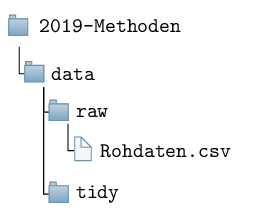
\includegraphics[width=0.5\linewidth]{figures/chap3-data-folder} \end{center}

Um die Daten einzulesen verwenden wir das Paket \texttt{tidyverse}, die
wir später genauer kennen lernen werden. Sie enthält viele nützliche
Funktionen zur Arbeit mit Datensätzen. Zudem verwende ich das Paket
\texttt{here} um relative Pfade immer von meinem Arbeitsverzeichnis aus
angeben zu können.\footnote{Das ist notwendig, da dieses Skript in R
  Markdown geschrieben ist und das Arbeitsverzeichnis automatisch auf
  den Ordner ändert, in dem das .Rmd file liegt. Mehr Information zum
  Schreiben von R Markdown finden Sie im Anhang. Dieser wird auch in der
  Vorlesung besprochen.}

\begin{Shaded}
\begin{Highlighting}[]
\KeywordTok{library}\NormalTok{(tidyverse)}
\KeywordTok{library}\NormalTok{(here)}
\end{Highlighting}
\end{Shaded}

Nehmen wir an, die Datei \texttt{Rohdaten.csv} sähe folgendermaßen aus:

\begin{verbatim}
Auto,Verbrauch,Zylinder,PS
Ford Pantera L,15.8,8,264
Ferrari Dino,19.7,6,175
Maserati Bora,15,8,335
Volvo 142E,21.4,4,109
\end{verbatim}

Wie in einer typischen csv Datei sind die Spalten hier mit einem Komma
getrennt. Um diese Datei einzulesen verwenden wir die Funktion
\texttt{read\_csv} mit dem Dateipfad als erstes Argument:

\begin{Shaded}
\begin{Highlighting}[]
\NormalTok{auto_daten <-}\StringTok{ }\KeywordTok{read_csv}\NormalTok{(}\KeywordTok{here}\NormalTok{(}\StringTok{"data/raw/Rohdaten.csv"}\NormalTok{))}
\NormalTok{auto_daten}
\end{Highlighting}
\end{Shaded}

\begin{verbatim}
#> # A tibble: 4 x 4
#>   Auto           Verbrauch Zylinder    PS
#>   <chr>              <dbl>    <dbl> <dbl>
#> 1 Ford Pantera L      15.8        8   264
#> 2 Ferrari Dino        19.7        6   175
#> 3 Maserati Bora       15          8   335
#> 4 Volvo 142E          21.4        4   109
\end{verbatim}

Wir haben nun einen Datensatz in R, mit dem wir dann weitere Analysen
anstellen können. Nehmen wir einmal an, wir wollen eine weitere Spalte
hinzufügen (Verbrauch/PS) und dann den Datensatz im Ordner
\texttt{data/tidy} speichern. Ohne auf die Modifikation des Data Frames
einzugehen können wir die Funktion \texttt{write\_csv} verwenden um den
Datensatz zu speichern. Hierzu geben wir den neuen Data Frame als
erstes, und den Pfad als zweites Argument an:

\begin{Shaded}
\begin{Highlighting}[]
\NormalTok{auto_daten_neu <-}\StringTok{ }\KeywordTok{mutate}\NormalTok{(auto_daten, }\DataTypeTok{Verbrauch_pro_PS =}\NormalTok{ Verbrauch}\OperatorTok{/}\NormalTok{PS)}
\KeywordTok{write_csv}\NormalTok{(auto_daten_neu, }\KeywordTok{here}\NormalTok{(}\StringTok{"data/tidy/NeueDaten.csv"}\NormalTok{))}
\end{Highlighting}
\end{Shaded}

Es wird ein späteres Kapitel (und einen späteren Vorlesungstermin)
geben, in dem wir uns im Detail mit dem Lesen, Schreiben und
Manipulieren von Datensätzen beschäftigen.

\appendix


\chapter{Eine kurze Einführung in R Markdown}\label{markdown}

Hier gibt es eine kurze Einführung in \texttt{R\ Markdown}. Wir
beschränken uns dabei auf die grundlegende Idee von Markdown, da die
konkrete Syntax im Internet an zahlreichen Stellen wunderbar erläutert
ist und man das konkrete Schreiben am besten in der Anwendung lernt.

\section{Markdown vs.~R-Markdown}\label{markdown-vs.r-markdown}

Bei \texttt{Markdown} handelt es sich um eine sehr einfache
Auszeichnungssprache, d.h. eine Programmiersprache, mit der schön
formatierte Texte erstellt werden können und die gleichzeitig auch für
Menschen sehr einfach lesbar ist. Dateien, die in Markdown geschrieben
sind, sind gewöhnlicherweise an der Endung \texttt{.md} zu erkennen.

R-Markdown stellt man sich am besten als eine Kombination von Markdown
und R vor: R-Markdown Dateien, die immer durch die Dateiendung
\texttt{.Rmd} gekennzeichnet sind, bestehen sowohl aus Markdown-Code,
als auch aus R-Code. Das bedeutet, dass man sein Forschungsprojekt
gleichzeitig erklären und durchführen kann. Im Prinzip können ganze
Forschungspapiere in R-Markdown verfasst werden und damit vollständig
reproduzierbar gestaltet werden.

\section{Installation von R-Markdown}\label{installation-von-r-markdown}

Für den Fall, dass Sie mit R-Studio arbeiten brauchen Sie lediglich das
Paket \texttt{rmarkdown} zu installieren:

\begin{Shaded}
\begin{Highlighting}[]
\KeywordTok{install.packages}\NormalTok{(}\StringTok{"rmarkdown"}\NormalTok{)}
\end{Highlighting}
\end{Shaded}

Das Standardformat für R-Markdown Dokumente ist html. Wenn Sie aber auch
PDF Dokumente erstellen wollen, müssen Sie auf Ihrem Computer
\href{https://www.latex-project.org/}{LaTex} installieren. Hierfür
finden sich zahlreiche Anleitungen im Internet (z.B.
\href{https://www.latex-tutorial.com/installation/}{hier} oder
\href{https://www.latex-project.org/get/}{hier}).

\section{Der R-Markdown Workflow}\label{der-r-markdown-workflow}

\subsection{Ein neues R-Markdown Dokument
erstellen}\label{ein-neues-r-markdown-dokument-erstellen}

R-Studio macht es Ihnen sehr leicht R-Markdown Dokumente zu erstellen.
Klicken Sie einfach auf den Button \texttt{Neu} und wählen dort dann
\texttt{R\ Markdown} aus, wie auf folgendem Screenshot zu sehen ist:

\begin{center}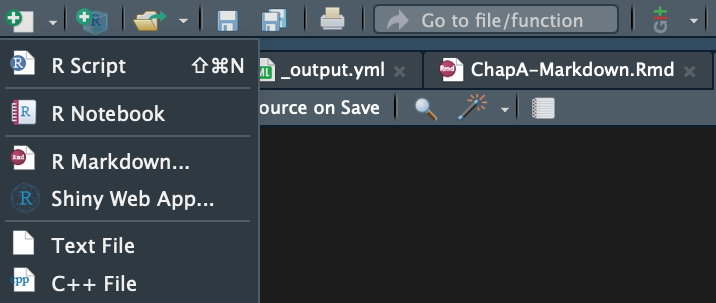
\includegraphics[width=0.75\linewidth]{/Users/claudius/work-claudius/general/paper-projects/packages/SocioEconMethodsR/figures/A-Markdown-NewFile} \end{center}

Im folgenden Fenster können Sie getrost die Standardeinstellungen so wie
vorgeschlagen belassen, da Sie alles später noch sehr leicht ändern
können.

Sie sehen nun eine Datei, das bereits einigen Beispielcode enthält und
damit schon einen Großteil der Syntax illustriert.

Ein R-Markdown Dokument besteht in der Regel aus zwei Teilen: dem
Titelblock und dem darunter folgenden Dokumentenkörper:

\begin{center}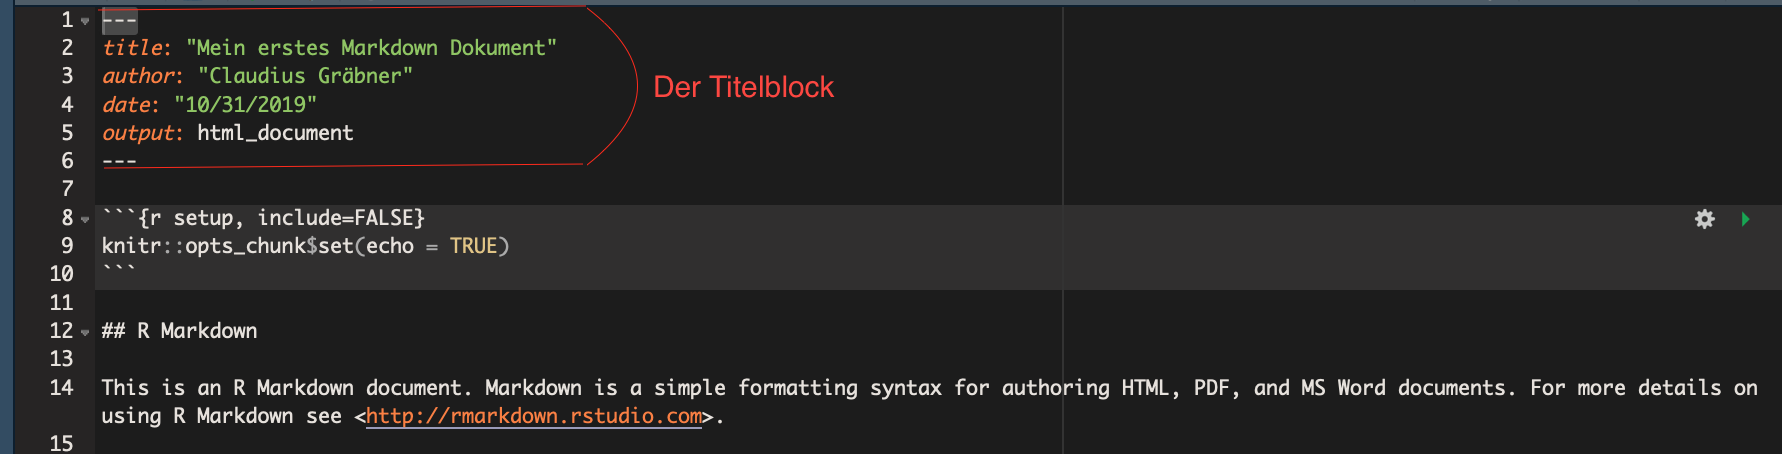
\includegraphics[width=0.75\linewidth]{/Users/claudius/work-claudius/general/paper-projects/packages/SocioEconMethodsR/figures/A-Markdown-Title} \end{center}

\subsection{Der Titelblock}\label{der-titelblock}

Der Titelblock ist immer durch zwei Zeilen mit dem Inhalt
``\texttt{-\/-\/-}'' oben und unten abgegrenzt. Die Syntax des
Titelblocks folgt der Sprache
\href{https://de.wikipedia.org/wiki/YAML}{YAML}, aber das hat wenig
praktische Relevanz. Im Titelblock werden alle globalen Einstellungen
für das Dokument vorgenommen. Für einfache Dokumente muss nur wenig an
den Standardeinstellungen geändert werden, aber im Laufe der Zeit werden
Sie merken, dass Sie über den YAML-Block Ihr Dokument zu ganz großen
Teilen individualisieren können. In der Regel finden Sie alle Antworten
durch Googlen, daher werde ich hier nicht weiter auf den Header
eingehen.

\subsection{Der Textkörper}\label{der-textkorper}

Der Textkörper besteht aus normalem Text, welcher in der Markdown Syntax
geschrieben ist, und so genannten \emph{Chunks}. Für die wirklich
einfache Syntax für normalen Text gibt es zahlreiche gute Anleitungen im
Internet, z.B. dieses eingängige
\href{https://rstudio.com/wp-content/uploads/2016/03/rmarkdown-cheatsheet-2.0.pdf}{Cheat
Sheet}.

Innerhalb der Chunks können Sie Code in einer beliebigen
Programmiersprache schreiben, insbesondere auch in R. Die Syntax
unterscheidet sich dabei überhaupt nicht von einem normalen R Skript.

Um einen Chunk zu Ihrem Dokument hinzuzufügen klicken Sie oben rechts im
Skripbereich auf `Insert' und wählen \texttt{R} aus:

\begin{center}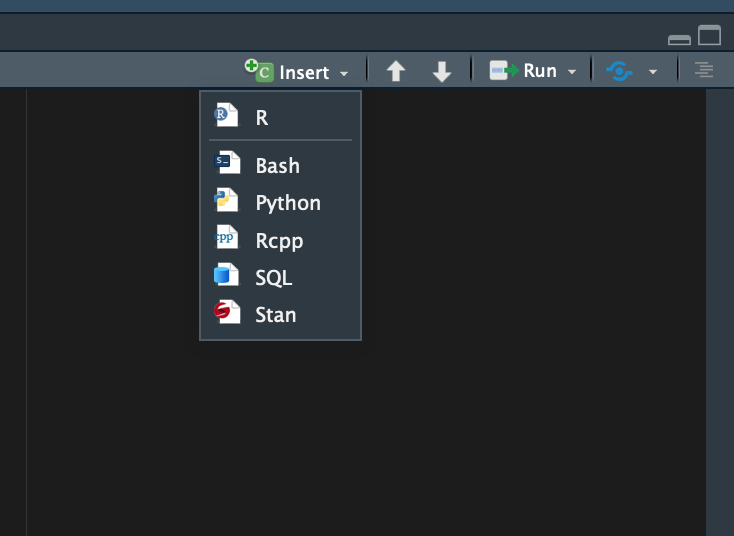
\includegraphics[width=0.75\linewidth]{/Users/claudius/work-claudius/general/paper-projects/packages/SocioEconMethodsR/figures/A-Markdown-Chunk1} \end{center}

Daraufhin wird an der Stelle des Cursors ein Chunk in Ihr Dokument
eingefügt. Dieser Chunk wird in der ersten und letzten Zeile durch
\texttt{\textasciigrave{}\textasciigrave{}\textasciigrave{}} begrenzt.
In der ersten Zeile wird zusätzlich innerhalb von geschweiften Klammern
die Programmiersprache des Chunks definiert:

\begin{center}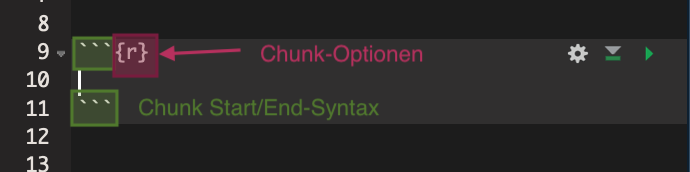
\includegraphics[width=0.75\linewidth]{/Users/claudius/work-claudius/general/paper-projects/packages/SocioEconMethodsR/figures/A-Markdown-Chunk3} \end{center}

Darüber hinaus kann das Ausführverhalten für den Chunk durch weitere
Argumente innerhalb der geschweiften Klammer weiter spezifiziert werden.

Häufig möchten Sie z.B., dass der Code im Chunk zwar im Dokument
angezeigt, aber nicht ausgeführt werden soll. Dies können Sie durch die
Option \texttt{eval=FALSE} erreichen. In diesem Fall sähe Ihr Chunk so
aus:

\begin{center}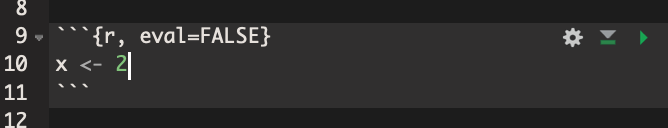
\includegraphics[width=0.75\linewidth]{/Users/claudius/work-claudius/general/paper-projects/packages/SocioEconMethodsR/figures/A-Markdown-Chunk4} \end{center}

In diesem Beispiel wird die Zuweisung \texttt{x\ \textless{}-\ 4} bei
der Kompillierung des Dokuments nicht ausgeführt.

Eine gute Übersicht über die Optionen, die Ihnen offen stehen, finden
Sie
\href{https://rstudio.com/wp-content/uploads/2015/03/rmarkdown-reference.pdf}{hier}
oder durch Googlen.

Sie können einzelne Chunks auch schon vor dem Kompillieren des Dokuments
ausführen indem Sie auf das Play-Zeichen oben links beim Chunk drücken.
Damit erhalten Sie eine Vorschau auf das Ergebnis.

\subsection{Kompillieren von
Dokumenten}\label{kompillieren-von-dokumenten}

Der Prozess, der aus dem Quellcode ihres Dokuments (also allem was in
der \texttt{.Rmd} Datei geschrieben ist) das fertige Dokument erstellt,
wird \emph{Kompillieren} genannt. Dabei wird aus dem \texttt{.Rmd}
Dokument ein gut lesbares \texttt{.html} oder \texttt{.pdf} Dokument
erstellt, wobei alle Chunks normal ausgeführt werden (es sei denn dies
wird durch die Option \texttt{eval=FALSE} verhindert).

Grundsätzlich gibt es zwei Möglichkeiten ein Dokument zu kompillieren:
über die entsprechende R-Funktion, oder über den Knit-Button in
R-Studio.

Die klassische Variante verwendet die Funktion \texttt{render()} aus dem
Paket \texttt{rmarkdown}. Die wichtigsten Argumente sind dabei die
folgenden: \texttt{input} spezifiziert die zu kompillierende
\texttt{.Rmd}-Datei, \texttt{output\_format} das für den Output
gewünschte Format\footnote{R-Markdown Dateien können in sehr viele
  verschiedene Formate kompilliert werden, das am häufigsten verwendete
  Format ist jedoch \texttt{html}. Eine Übersicht finden Sie
  \href{https://bookdown.org/yihui/rmarkdown/output-formats.html}{hier}.}
und \texttt{output\_file} den Pfad und den Namen der zu erstellenden
Outputdatei.

Wenn Sie also das Dokument \texttt{FirstMarkdown.Rmd} kompillieren
wollen und den Output unter \texttt{Output/OurMarkdown.html} als
html-Datei speichern wollen, dann können Sie das mit folgendem Code,
vorausgesetzt die Datei \texttt{FirstMarkdown.Rmd} liegt im Unterordner
\texttt{R}:

\begin{Shaded}
\begin{Highlighting}[]
\KeywordTok{render}\NormalTok{(}\DataTypeTok{input =} \StringTok{"R/FirstMarkdown.Rmd"}\NormalTok{, }\DataTypeTok{output_format =} \StringTok{"html"}\NormalTok{, }
    \DataTypeTok{output_file =} \StringTok{"output/FirstMarkdown.html"}\NormalTok{)}
\end{Highlighting}
\end{Shaded}

Weitere Informationen zu den Parametern finden Sie wie immer über die
\texttt{help()} Funktion. Alternativ können Sie auch den Button
\texttt{Knit} in der R-Studio Oberfläche verwenden. Das ist in der Regel
bequemer, lässt aber weniger Individualisierung zu.

\section{Relative Pfade in
Markdown-Dokumenten}\label{relative-pfade-in-markdown-dokumenten}

Der problematischste Teil beim Arbeiten mit R-Markdown ist der Umgang
mit relativen Pfaden. Um das Problem zu illustrieren nehmen wir einmal
folgende Ordnerstruktur an, wobei der Ordner \texttt{MarkdownProject}
unser Arbeitsverzeichnis ist:

\begin{center}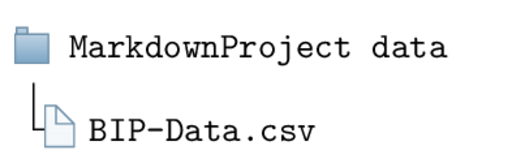
\includegraphics[height=0.25\textheight]{/Users/claudius/work-claudius/general/paper-projects/packages/SocioEconMethodsR/figures/A-Markdown-Ordnerstruktur} \end{center}

Das Problem ist nun, dass wenn Sie eine R-Markdown Datei kompillieren,
diese Datei alle Pfade \textbf{nicht} ausgehend von Ihrem
Arbeitsverzeichnis interpretiert, sondern vom \emph{Speicherort} der
\texttt{.Rmd}-Datei. Das ist natürlich hochproblematisch, denn stellen
Sie sich vor, Sie möchten in Ihrem R-Markdown-Skript die Datei
\texttt{data/BIP-Data.csv} einlesen. Normalerweise würden Sie dafür den
folgenden Code verwenden:

\begin{Shaded}
\begin{Highlighting}[]
\NormalTok{bip_data <-}\StringTok{ }\KeywordTok{fread}\NormalTok{(}\StringTok{"data/BIP-Data.csv"}\NormalTok{)}
\end{Highlighting}
\end{Shaded}

Zwar würde der Code in einem R-Skript, z.B. in \texttt{R/R-Skript.R}
perfekt funktionieren. In einem R-Markdown Dokument, das nicht im
Arbeitsverzeichnis direkt gespeichert ist, jedoch nicht. Da in
R-Markdown-Dokumenten alle Pfade relativ des Speicherorts des Dokuments
interpretiert werden, müssten wir hier schreiben:\footnote{Mit
  \texttt{../} bewegt man sich bei einem relativen Pfad einen Ordner
  nach oben.}

\begin{Shaded}
\begin{Highlighting}[]
\NormalTok{bip_data <-}\StringTok{ }\KeywordTok{fread}\NormalTok{(}\StringTok{"../data/BIP-Data.csv"}\NormalTok{)}
\end{Highlighting}
\end{Shaded}

Das wäre allerdings unschön, weil wir dann unterschiedlichen Codes in
Skripten und in R-Markdown-Dokumenten verwenden müssten und das Ganze
dadurch deutlich verwirrender werden würde.

Es wäre also schön, wenn R automatisch wüsste, was das
Arbeitsverzeichnis des aktuellen Projekts ist und dieses automatisch
berücksichtigt, unabhängig davon ob wir mit einem \texttt{.R} oder
\texttt{.Rmd} Dokument arbeiten und wo dieses Dokument innerhalb unserer
Projekt-Struktur gespeichert ist.

Zum Glück können wir genau das mit Hilfe des Pakets
\href{https://github.com/jennybc/here_here}{here} erreichen.\footnote{Tatsächlich
  ist \texttt{here} dermaßen praktisch, dass ich empfehle grundsätzlich
  alle Pfade in jedem Projekt - ob R-Markdown oder nicht - mit Hilfe von
  \texttt{here} anzugeben.} Das Paket enthält eine Funktion
\texttt{here()} die als Argument einen Dateinamen oder einen relativen
Pfad akzeptiert, und daraus einen absoluten Pfad auf dem Computer, auf
dem der Code gerade ausgeführt wird, konstruiert.

Wir können also unseren Code von oben einfach folgendermaßen
umschreiben:

\begin{Shaded}
\begin{Highlighting}[]
\NormalTok{bip_data <-}\StringTok{ }\KeywordTok{fread}\NormalTok{(}\KeywordTok{here}\NormalTok{(}\StringTok{"data/BIP-Data.csv"}\NormalTok{))}
\end{Highlighting}
\end{Shaded}

In dieser Form funktioniert er sowohl in \texttt{.R} als auch
\texttt{.Rmd} Dateien ohne Probleme.

\begin{quote}
\textbf{Hinweis I:} Die Funktion \texttt{here()} verwendet verschiedene
Heuristiken um das Arbeitsverzeichnis des aktuellen Projekt
herauszufinden. Darunter fällt auch das Suchen nach einer
\texttt{.Rproj} Datei. Überhaupt funktionieren die Heuristiken in der
Regel wunderbar und können für Ihren konkreten Fall über die Funktion
\texttt{dr\_here()} angezeigt werden. Um ganz sicherzugehen sollte man
aber immer in das Arbeitsverzeichnis eine Datei \texttt{.here} ablegen.
Diese kann manuell, oder über die Funktion \texttt{set\_here()},
erstellt werden.
\end{quote}

\begin{quote}
\textbf{Hinweis II:} Die Verwendung von \texttt{here()} ist essenziell,
wenn Ihre R-Markdown Dokumente auf mehreren Computern funktionieren
sollen. Daher ist die Verwendung in den Arbeitsblättern
\textbf{verpflichtend}.
\end{quote}

\section{Weitere Quellen}\label{weitere-quellen}

Eine gute Übersicht über die häufigsten Befehle enthält dieses
\href{https://rstudio.com/wp-content/uploads/2016/03/rmarkdown-cheatsheet-2.0.pdf}{Cheat
Sheet}. Eine sehr umfangreiche Einführung bietet das Online-Buch
\href{https://bookdown.org/yihui/rmarkdown/}{R Markdown: The Definitive
Guide}. Aber auch darüber hinaus finden sich im Internet zahlreiche
Beispiele für die R-Markdown-Syntax. Dieses Skript wurde übrigens in
\href{https://bookdown.org/yihui/bookdown/}{R Bookdown}, einer
Erweiterung von R-Markdown für Bücher, geschrieben.

\bibliography{book.bib,packages.bib}



\end{document}
